%% ----------------------------------------------------------------
%% Thesis.tex -- main
%% ---------------------------------------------------------------- 

\documentclass[a4paper, 10pt, oneside]{memoir}
%% Use the option citeauthor to be able to use citet. The default cite will still work.
\usepackage[labelformat=simple]{subcaption}
\usepackage[citeauthor]{basilea}


\usepackage{graphicx}

%\usepackage{pdflscape}
%\usepackage{tikz}
%\usepackage{changepage}

%\usepackage{pgfgantt}

%\usepackage{tikz,lipsum,lmodern}
\usepackage[most]{tcolorbox}

% Some additional math symbols
\usepackage{amsmath}
\usepackage{stmaryrd}

%\usepackage{afterpage} % footnote in image
\usepackage{float} % float with H

%\usepackage{wrapfig} % wrap text around figures
%\usepackage{algorithm}
%\usepackage{algpseudocode}


\newcommand{\norm}[1]{\left\lVert#1\right\rVert}
\newcommand{\snry}{$\text{SNR}_y$ }
\newcommand{\snrh}[1]{\footnotesize \textbf{\snry #1 dB}}

\newcommand{\visualresult}[3]{
\begin{figure}[H]
  \centering
	\caption{#3 reconstruction for \snry #2 dB.}
  \includegraphics[width=0.16\textwidth]{#1/#2/#1_#2_1.png}
  \hfill
  \includegraphics[width=0.16\textwidth]{#1/#2/#1_#2_2.png}
	\hfill
  \includegraphics[width=0.16\textwidth]{#1/#2/#1_#2_3.png}
	\hfill
  \includegraphics[width=0.16\textwidth]{#1/#2/#1_#2_6.png}
	\hfill
  \includegraphics[width=0.16\textwidth]{#1/#2/#1_#2_9.png}
	\hfill
  \includegraphics[width=0.16\textwidth]{#1/#2/#1_#2_10.png}
\end{figure}
}

\newcommand{\visualresults}[1]{
  \subsubsection{Clean Test Images}
\begin{figure}[H]
  \centering
  \hfill
  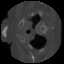
\includegraphics[width=0.16\textwidth]{clean/clean_1.png}
  \hfill
  
\includegraphics[width=0.16\textwidth]{clean/clean_2.png}
  \hfill
  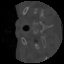
\includegraphics[width=0.16\textwidth]{clean/clean_3.png}
  \hfill
  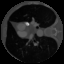
\includegraphics[width=0.16\textwidth]{clean/clean_6.png}
  \hfill
  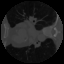
\includegraphics[width=0.16\textwidth]{clean/clean_9.png}
  \hfill
  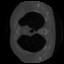
\includegraphics[width=0.16\textwidth]{clean/clean_10.png}
  \hfill
  \caption{Clean test images.}
\end{figure}

	\subsubsection{Baseline Algorithms}
  \visualresult{fbp}{#1}{FBP}
  \visualresult{bm3d\_sino}{#1}{BM3D sino}
  \visualresult{bm3d\_reco}{#1}{BM3D reco}
  \visualresult{unet}{#1}{U-Net}

  \subsubsection{GAT-Denoiser Models}
  \visualresult{gat}{#1}{GAT}
  \visualresult{conv\_gat}{#1}{Conv + GAT}
  \visualresult{gat\_unet}{#1}{GAT + U-Net}
  \visualresult{conv\_gat\_unet}{#1}{Conv + GAT + U-Net}

}
%% ----------------------------------------------------------------

\title				{Graph Denoising for Molecular Imaging}
\thesistype			{Master's Thesis}

\department 		{Department of Mathematics and Computer Science}
\faculty			{Natural Science Faculty of the University of Basel}
\research		    {Signals and Data Group}

\examiner    		{Prof. Dr. Ivan Dokmanić}
\supervisor  		{Dr. Valentin Debarnot}

\authors     		{Cédric Mendelin}
\email				{cedric.mendelin@stud.unibas.ch}
\immatriculnr		{2014-469-274}

\date				{12.06.2022}

% switch here for the German logo to logo-de
\ulogo				{Template/logo-en} 


%% ----------------------------------------------------------------
\begin{document}

\selectlanguage{english}

\thesisfront
\maketitle
\pagestyle{thesis}
%% ----------------------------------------------------------------
% !TEX root = ../Thesis.tex
\chapter{Acknowledgments}
So Long, and Thanks for All the Fish. And the template.
%% ----------------------------------------------------------------
% !TEX root = ../Thesis.tex
\chapter{Abstract}
This thesis discusses the thesis template using some examples of the Turing Machine.
%% ----------------------------------------------------------------
\thesistoc
%% ----------------------------------------------------------------
%\thesisnomencl
%% ----------------------------------------------------------------
\thesismain

\chapter{Assessment criteria}
Written report including: 
\begin{itemize}
    \item Contents of the Master's Thesis project
    \item Project plan
    \item summary of relevant related work
\end{itemize}

\chapter{Foundation}



\textbf{General Questions}
\begin{itemize}
    \item Difference Graph Learning and Graph Representation
    \item Eigenvalues
    \item First-order Chebyshev
    \item Connection to CryoEm
    \item Benchmarking and Dataset
\end{itemize}

\textbf{Questions GCN:}
\begin{itemize}
    \item During feature propagation, only node features are considered.
    \item Spectral Analysis Chapter
    \item Degree of = A + I same as $\hat{D} = D + I$, not 2 times with self loop?
\end{itemize}

\section{Introduction to Graph Learning}

Graph Representational Learning
\footnote{https://towardsdatascience.com/introduction-to-graph-representation-learning-a51c963d8d11}


\subsection{Spectral graph theory}
Spectral graph theory \cite{SpectralGraphTheory} deals with learning properties and characteristics of graphs, in regard to
the graphs eigenvalues and eigenvectors. 

\subsection{Graph deep Learning}
Deep Learning with graphs.
\textbf{TODO: write more}


\section{Noise}
A noisy observation is defined as:
$y_n = y + \eta$

\subsection{Denoising}
When we talk from denoising, we want to reconstruct the true observation 
from a given noisy observation. This reconstruction is done via averaging, which can be performed
locally, by the calculus of variations or in the frequency domain.

\subsubsection{Non local means}
Non local means is a state-of-the-art image denoising method \cite{noneLocalMean}.
In the name of the method are two important concepts, namely the \textit{mean}
and \textit{non local}.

For a given noisy image $v$, the denoised image is defined as:
\begin{equation}
    NL[v](i) = \sum{w(i,j)v(j)}
\end{equation}

where $w(i,j)$ is the weight between pixel $i$ and $j$ and fulfils two conditions:
\begin{itemize}
    \item $0 \le w(i,j) \le 1$
    \item $\sum_j{w(i,j) = 1}$
\end{itemize}

Without going into detail, the weight can be seen as a similarity measure of the two pixels.
Moreover, are these similarities calculated over square neighbourhoods of the two pixels.
Similar pixel neighbourhoods have a large weight and different neighbourhoods have a small weight.

More general, the denoised image pixel $i$ is computed 
as an weighted average of all pixels in the image, therefore, in a non local way.

\section{Graph Foundations}
A graph is defined as  $G = \langle V,E \rangle$, where $V$ is a set of 
vertices (or nodes) and $E$ is a set of edges (or links). Edges are 
defined as a set of tuples $\langle i,j \rangle$, where $i$ and $j$ determine the 
index of the vertices in the graph.

\subsection{Adjacency Matrix}

The adjacency Matrix of $G$ is then defined as follows:
\begin{equation}
    A_{ij} =    
    \begin{cases}
        %1  & \text{if } \norm{\biggl y_i - y_j \biggr} < \tau\\
        1  & \text{if } \langle i,j \rangle \in E \\
        0, & \text{otherwise}
    \end{cases}
\end{equation}

\subsubsection{k-hop neighbourhood}

\subsection{Degree Matrix}

The degree Matrix of $G$ is defined as follows:
\begin{equation}
    D_{ij} =    
    \begin{cases}
        %1  & \text{if } \norm{\biggl y_i - y_j \biggr} < \tau\\
        deg(v_i)  & \text{if } i = j \\
        0, & \text{otherwise}
    \end{cases}
\end{equation}

Where $deg(v_i)$ is the degree of the node, formally the number of incoming edges of node $v_i$.

\subsubsection{Adjacency normalization}
We starting calculating with Matrix A, it is sometimes necessary to normalize.
With the degree Matrix $D$ and Adjacency Matrix $A$, we have all information we need.
Mostly, we want to normalize, such that our rows sum to 1.
\begin{equation}
    A_{rownorm} = D^{-1} A
\end{equation}

But we can achieve the same for columns, we just need to swap the two matrices:
\begin{equation}
    A_{colnorm} = A D^{-1}
\end{equation}

And a final, a probably the most useful normalization, is the symmetric normalization:

\begin{equation}
    A_{sym} =  D^{-\frac{1}{2}} A D^{-\frac{1}{2}}
\end{equation}

\textbf{TODO: Add some nice example}

\subsection{Graph Laplacian}
The graph Laplacian is defined as follows:
\begin{equation}
    L = D - A
\end{equation}


\subsubsection{Normalized Graph Laplacian}

Symmetric normalized: $L_{sym} = I - D^{-\frac{1}{2}} A D^{-\frac{1}{2}}$
Random walk normalized: $L_{rw} = I - D^{-1} A$

\subsubsection{Normalized Graph Laplacian eigendecomposition}

\begin{equation}
    \begin{aligned}
        L_{sym} =U \Lambda U^T \\
        U = [u_0, \ddots, u_{N-1}] \in R^{N x N}\\
        \Lambda = diag ( [\lambda_0, \ddots, \lambda_{N-1}] ) \in R^{N x N}
    \end{aligned}
\end{equation}

In this scenario, Eigenvectors are also known as \textit{graph Fourier modes}
and eigenvalues are known as the \textit{spectral frequencies}.

Moreover, with the Graph Fourier Transform, we can calculate these values from a symmetric
graph Laplacian.

\subsection{Graph Properties}

\subsubsection{Directed vs. undirected vs. weighted}

\subsubsection{Dense and sparse Graph}
A dense graph is a graph, where the number of edges in close to the maximal number of edges.
Contrarily, a sparse graph only consists of a few edges.



\subsection{Node Properties}
\subsection{Edge Properties}

\subsection{Graph Construction}
\textbf{TODO: KNN}



\section{Graph Denoising}
Data acquired by Real-world observations are often noisy, which can lead to poor 
performance on data analysis tasks. This observed data can already be in the form of a graph,
or a graph can be easily constructed. This resulting graph is what we call
a noisy graph, as it includes the noise from the observation.

Graph denoising is the task to reconstruct the original graph from a noisy one.
Therefore, graph denoising can be seen as a pre-processing step, where noisy data is filtered.

Denoising in general has often to do with averaging \cite{noneLocalMean}
 and graphs are  a well suited data structure for this task.

\subsection{Noisy Graph}
For every noisy graph, there exists an original graph $G = \langle V,E \rangle$.

The noisy graph can be defined as follows:
\begin{equation}
    \begin{aligned}
        G_{noisy} = \langle V,E_{noisy} \rangle \\ 
        \text{ where }  E_{noisy} = E \setminus  E^{-} \cup  E^{+} \\ 
        \text{ and } E^{-} \subseteq E  ,  E^{+} \cap E = \emptyset
    \end{aligned}
\end{equation}

Basically, the noisy graph consists of the same vertices as the original graph. From
the original graphs edges, some are removed (denoted by $E^{-}$) and some new edges are added
(denoted by $E^{+}$).

The adjacency Matrix of $G_{noisy}$ is then defined as follows:
\begin{equation}
    \bar{A}_{ij} =    
    \begin{cases}
        %1  & \text{if } \norm{\biggl y_i - y_j \biggr} < \tau\\
        1  & \text{if } \langle i,j \rangle \in E_{noisy} \\
        0, & \text{otherwise}
    \end{cases}
\end{equation}

The task of graph denoising, can therefore be written as:
\begin{equation}
    \bar{A} \xrightarrow[method]{Graph denoising} \tilde{A} \approx A
\end{equation}

Where $\bar{A}$ denotes the noisy input graph, $\tilde{A}$ the denoised
 graph and $A$ the original graph.


\subsection{Graph link prediction}
Link prediction is a task in Graph learning. 
The idea is to predict the existence of a link (edge) between two nodes.
The task can be formulated as a missing value estimation task. A model $M_p$ is learned
from a given set of observed edges. The model finally maps links to probabilities:


\begin{equation}
    M_p : E^{\prime} \rightarrow [0,1]
\end{equation}

Where $E^{\prime}$ is the set of potential links.


We define $U$ as the set of all possible vertices of $G$, therefore $E \subseteq U$.
Obviously, one could see Graph denoising as a link prediction problem.

The difference is, that in link prediction, we learn a model from a set of observed links 
$E_{observed} \subseteq E$ and in Graph denoising we learn the model from 
$E_{observed} \subseteq U$. 

On could also say that link prediction problems are a subset of graph denoising problems.


\section{Graph Laplacian}

\section{Deep Learning on Graphs}

\subsection{Graph Convolutional Network}
Graph Convolutional Networks (GCN) \cite{GCN} can be used for many tasks in the field 
of Graph Learning, such as node classification or link prediction. 
Basically, with GCN, a new feature representation is iteratively learned for the node features.

The basic concept is as follows:
For a given graph $G = \langle V,E \rangle$, with node features $X^{N x D}$ and adjacency Matrix $A$
where $N$ denotes the number of nodes and $D$ the number of node input attributes,

a novel node representation $Z^{N x F}$ will be learned, where $F$ is the number of output features.

$Z$ will be learned within a neural network, and every layer can be written by the following, non-linear function:

\begin{equation}
    \begin{aligned}
        H^{l + 1} = f( H^l, A), \\
        \text{with } H^0 = X \text{ and } H^L = Z, 
    \end{aligned}
\end{equation}

where $L$ is the number of layers in the neural network.
The model only differ in the choice of $f(\cdot,\cdot)$.

We are ready to define our first GCN. To keep it simple, $f(\cdot,\cdot)$ will be defined as the following:
\begin{equation}
    f( H^l, A) = \sigma (A H^l W^l)
\end{equation} 

Where $\sigma ( \cdot )$ is a non-linear activation function, such as ReLU and $W^l$ is
a weight Matrix of the layer $l$ of the neural network. As \cite{GCN} could show during experiments,
this choice of $f(\cdot,\cdot)$ is already very powerful and leads to state-of-the-art results.

\subsubsection{Renormalization trick}

With this model, we do have two problems and need to refine it further.
First of all, with the multiplication of $A$, we average over the neighbour nodes but
will ignore the node itself. Therefore, self-loops will be added to $A$.
The second problem is, that A is not normalized and if therefore, when multiplying with $A$,
the features of the nodes will change it scale. Therefore, we need to normalize $A$
such that all rows sum to one. This can be done with a simple multiplication with the D.

These two steps are called the Renormalization trick \cite{GCN}
First of all, we can simple add the self-loops by adding the Identity Matrix to $A$, 
$\hat{A} = A + I$ and $\hat{D}$ is the degree Matrix of $\hat{A}$.
Now, we can achieve a symmetric normalization by multiplying $D^{-\frac{1}{2}} A D^{-\frac{1}{2}}$.

And finally, we can put all things together, and replace $A$ in the original equation:
\begin{equation}
    f( H^l, A) = \sigma (\hat{D}^{-\frac{1}{2}} \hat{A} \hat{D}^{-\frac{1}{2}} H^l W^l)
\end{equation} 


\subsubsection{Simple Graph Convolutional Network}
Simple Graph Convolutional Network (SGC) \cite{simpleGCN} proposed a simplified version of GCN.
They could verify their hypothesis, that GCN is dominated by the local averaging step and the non-linear 
activation function between layers do not contribute to much to the success of GCN.

This makes the calculation simpler. We denote $S = \hat{D}^{-\frac{1}{2}} \hat{A} \hat{D}^{-\frac{1}{2}} $
and can use the fact that in every layer of the neural network, the same computation will take place.

\begin{equation}
    \begin{aligned}
        Z = S \ddots S X W^1 W^2 \ddots W^L \\
        Z = S^L X W^1 W^2 \ddots W^L \\
        Z = S^L X W    
    \end{aligned}
\end{equation}

where $W$ is the matrix of all vector weights.



\subsubsection{Link go Graph Laplacian:}

In the section, we will have a look at the connection between SGC and Graph Laplacian.

We can define $x \in R^n$ as our signals and define the Fourier transform as $\hat{x} = U^T x$
and the inverse as $x = U\hat{x}$. 
With the transform, we can easily switch between spatial and Fourier(spectral) domain.

Further, we can define the graph convolution operation between signal $x$ and filter $g$.

\begin{equation}
    g \star x = U((U^T g) (U^T x)) = U \hat{G} U^T x,
\end{equation}

where $\hat{G}$ is a diagonal matrix where the elements are the 
spectral filter coefficients (eigenvalues?)

The graph convolution can be approximated by the $k$-th order polynomials of Laplacians:

\begin{equation}
    \approx \sum_{i=0}^{k} \Delta^i x = U \left ( \sum_{i=0}^{k}  \Theta_i \Lambda^i \right ) U^T x,
\end{equation}

where $\Delta = D - A$ and $\Theta_i$ are 
filter coefficients which correspond to polynomials of the Laplacian eigenvalues,
 $\hat{G} = \sum_i \Theta_i \Lambda^i$


 In the original \cite{GCN} paper, the approximation is done with $k = 1$ 
 \begin{equation}
     g \star x = \Theta (I + D^{-\frac{1}{2}} A D^{-\frac{1}{2}} )x,
 \end{equation}

, where \citet{GCN} further applies the renormalization trick, ending up replacing
$I + D^{-\frac{1}{2}} A D^{-\frac{1}{2}}$ with $\hat{D}^{-\frac{1}{2}} \hat{A} \hat{D}^{-\frac{1}{2}}$.

$I + D^{-\frac{1}{2}} A D^{-\frac{1}{2}}$ is also called first-order Chebyshev filter.

\footnote{https://towardsdatascience.com/spectral-graph-convolution-explained-and-implemented-step-by-step-2e495b57f801}

not read currently:
\footnote{https://towardsdatascience.com/tutorial-on-graph-neural-networks-for-computer-vision-and-beyond-part-2-be6d71d70f49}

%\chapter{Papers - Foundation}

\section{Maths Foundation}
\subsection{Hilbert Space}
\subsection{SO(3), S,}
\subsection{LIE Group?}
\subsection{Principle component analysis - PCA}
\subsection{Local PCA}
\subsection{K-means}
\subsection{K-nearest neighboors Graph construction}
\subsection{Fourier domain}

\subsection{Graph Fourier transform}


\section{Graph Foundation}
\subsection{Curvature}
\subsection{Graphlets}
\subsection{Geodesic distance}
\subsection{Manifold Assumption}
\subsection{Point Cloud}
\subsection{Laplace}
\subsection{Walk Pooling}
\subsection{Link prediction}
\subsection{Katz Index}

\subsection{Eigenvector centrality}
\subsection{NN forward passing}
\begin{equation}
    H^{i + 1} = \sigma ( W^i H ^i + b^i)
\end{equation}
\footnote{https://towardsdatascience.com/understanding-graph-convolutional-networks-for-node-classification-a2bfdb7aba7b}

\subsection{NN activation functions}
\subsection{Drops after layer}

\subsection{Hyper Graphs}
\subsection{Power Iterations}
\subsection{Manifold Learning}
\subsection{Signal Processing}
\subsection{Nonlinear dimensionality reduction}


\section{Diffusion Maps:}
\citet{diffusionMaps}
\cite{diffusionMaps}

Dimensionality reduction:
In essence, the goal is to change the representation of data sets, originally in a form involving a large number of variables, into a
low-dimensional description using only a small number of free parameters.

meaningful structures in data sets:
Analogous to the problem of dimensionality reduction is that of finding meaningful structures in data sets. The idea here is slightly
different and the goal is to extract relevant features out of the data in order to gain insight and understanding of the
phenomenon that generated the data.

Markov Chain:

Random walk:

PageRank:
Stationary distribution of random walk

Kernel eigenmap methods:
- local linear embedding
- Laplacian eigenmaps,
- hessian eigenmaps
- local tangent space alignement

The remarkable idea emerging from these papers is that eigenvectors of Markov matrices can be thought of as coordinates
on the data set. Therefore, the data, originally modeled as a graph, can be represented (embedded) as a cloud of points
in a Euclidean space.
two major advantages over classical dimensionality redution (PCA, MDS):
The first aspect is essential as most of the time, in their original form, the data points do not lie on
 linear manifolds.
 The second point is the expression of the fact that in many
applications, distances of points that are far apart are meaningless, and therefore need not be preserved.

Unnormalized Graph Laplacian:
$L = D - W$

Normalized Graph Laplacian construction:
$L_{sym} = D^{-1/2}LD^{-1/2} = I - D^{-1/2}WD^{-1/2} $
$L_{rw} = D^{-1}L = I - D^{-1}W $

Markov chain has a stationary distribution.
If graph is connected, stationary is unique.
If X is finite, chian is ergodic.

Diffusion distance:
Diffusion map $\psi$ embeds the data into the Euclidean space so that in this space, the Euclidean
distance is equal to the diffusion distance.

Laplace–Beltrami operator on manifolds

What are diffusion maps

\subsection{Vector Diffusion Maps (VDM)}

\cite{vectorDiffusionMaps}
VDMis a mathematical and algorithmic generalization of diffusion maps
and other nonlinear dimensionality reduction methods, such as LLE, ISOMAP,
and Laplacian eigenmaps. While existing methods are either directly or indirectly
related to the heat kernel for functions over the data, VDM is based on
the heat kernel for vector fields.

Main concept:
Edge consists of weight and linear orthogonal transformation.
If linear orthogonal transformation is big, nodes are more like to be equal.
If small, there are different

Diffusion is calculated on vectors fields, where tangets are mapped to the manifold.
A way to globally connect Local PCAs.

\textbf{SNR: signal-to-noise-ratio}


LLE:
ISOMAP:
Laplacian eigenmaps:


\subsection{Riemannian Manifold Assumption:}
One of the main objectives in the analysis of a high-dimensional large data set
is to learn its geometric and topological structure. Even though the data itself is
parametrized as a point cloud in a high-dimensional ambient space $R^p$, the correlation
between parameters often suggests the popular “manifold assumption” that
the data points are distributed on (or near) a single low-dimensional Riemannian
manifold Md embedded in Rp, where d is the dimension of the manifold and
$d << p$.


\subsection{Multi-Frequency Vector Diffusion Maps (MFVDM)}
\cite{multiDiffusionMaps}
\textbf{For a direct link between manifold embedding and tomography, very close to what Ivan explained this morning.
If we have a graph denoising method, we will need to compare with this approach 
(or the original vector diffusion maps).}

Basically same as VDM, but with multiple frequencies per edge.

Diffusion maps (DM) only consider scalar weights over the edges and the vector
diffusion maps (VDM) only take into account consistencies
of the transformations along connected edges using only one
representation of $SO(2)$, i.e. $e^{ia_{i,j}}$ . In this paper, we generalize
VDM and use not only one irreducible representation,
i.e. $k = 1$, but also higher order $k$ up to $k_{max}$.


\section{Graph Laplacian Tomography From Unknown Random Projections}
\textbf{A reference that I already mentioned in the first mail:
standard approach that we need to compare with. 
Maybe their setting (2D tomography with unknown angle) is a good setting to start with.
}

\section{denoising}
Recover original image from noisy observation.
Is Achieved by averaging.

- classical local smoothing filters:
    - gaussian filters
    - anisotropic filters
    - Total Variation minimization
    - neighborhood filters

- neighborhood filters (review of image denoising)
- non local means
- functions adapted kernels (nonlinear independent component analysis)


\section{Non-local means}
Image denoising accurately done.

Better performance, when algorithms tries to correct noise rather than separate noise
from original image.

Compares similar pixel neighborhoods and assign large weighted for similar pixels.




\section{Learning to Drop}
Graph denoising


\section{WalkPooling}
Image denoising

\section{Point Clouds}
\subsection{Dynamic graph Cnn for learning on point clouds}
One of the few reference related to graph neural network and learning of graph structure. 


\subsection{CryoEm and related}
2. Estimation of Orientation and Camera Parameters from Cryo-Electron Microscopy Images with Variational Autoencoders and Generative Adversarial: 

learning framework where the manifold embedding is estimated.

3. Computational Methods for Single-Particle Cryo-EM: 
review around cryo-EM. 

This reference doesn't talk about manifold embedding, but it is a nice one if you want to know more about 
the acquisition system and standard approaches to solve the cryo-EM problem.


3.bis) Single-Particle Cryo-Electron Microscopy: 
another review similar to the previous one. The section "Mathematical frameworks for cryo-EM data analysis" 
and especially the subsection MRA (multireference alignement) introduce 
a toy model that is related to cryo-EM and where the symmetries are of importance. 

4. Bispectrum Inversion with Application to Multireference Alignment: 
for a paper that introduce several algorithms to solve MRA.
\chapter{Introduction}
\label{sec:introduction}

Inverse problems refer to the process, which, from observed data, derive a model that produces
the data. They are widely used throughout different science directions, such as Machine Learning (ML),
signal processing, computer vision, natural language processing and many more.

In recent years, Graphs got a lot of attention in ML and are one of the most promising research areas.
Graphs are a well suited data structure, simple but with high expressiveness 
and, therefore, well suited in ML.

Cryo-electron microscopy (cryo-EM), gained a lot of attention in recent years. 
Due to ground-breaking improvements regarding hardware and data processing, the field of research
has highly improved. In the year 2017, the pioneers in the field of cryo-EM even got the 
Nobel Prize in Chemistry\footnote{https://www.nobelprize.org/prizes/chemistry/2017/press-release/}
Today, using cryo-Em many molecular structures can be displayed with near-atomic resolution.

\bigskip

The following report resulted as the Master Thesis Preparation report. During the six weeks project, 
the aim was to familiarize with the research direction, build up the mathematically foundation needed 
for the Thesis itself and define the project content and an overall project plan.

\bigskip

The report is structured as the following:
In chapter~\ref{sec:foundation}, the overall foundation for the Master Thesis will be given, focusing 
on Graph Learning, Graph Denoising, some mathematically methods and definitions as well as
 a short introduction to cryo-EM.
Chapter~\ref{sec:preliminariesProblem} is dedicated to the problem setup and some preliminaries of the problem. 
Moreover, the base idea of the Master Thesis is defined.
Up to this point, the underlying problem has been defined and some related work can be given in chapter~\ref{sec:relatedWork}.





\chapter{Imaging methods}
\label{sec:imaging}

In the current chapter, imaging methods \textit{computed tomography} and 
\textit{cryo-electron microscopy} (cryo-EM) will be introduced. 
Further, their observation model is defined in a mathematically way and their reconstruction is observed.
Application of cryo-EM is the major motivation for the Master Thesis, 
as the problem is not easy to solve due to dealing with enormous noise and other difficulties.


\section{Computed tomography}
Computed tomography is a well established imaging method.
Using X-ray source, fan shaped beams are produced which scan the imaging object,
resulting in many measurements taken over straight lines \cite{computedTomography}.

\paragraph{Tomography reconstruction:}
Tomographic reconstruction\cite{tomographicReconstruction} is a popular inverse problem. 
The aim is to reconstruct an imaged object from observed measurements.
The reconstruction object can be in two-dimension (2D) or in three-dimension (3D). 

\begin{tcolorbox}[colback=red!5!white,colframe=red!75!black]
    In the Master Thesis, the focus on computed tomography will be on 2D case, which is called \textit{classical tomography reconstruction}.
\end{tcolorbox}

\paragraph{2D tomographic reconstruction:}

Mathematically, the observed measurements can be defined as follows:

\begin{equation}
    \label{eq:2Dreconstruction}
    \begin{aligned}
        y_i[j] &= R(x, \theta_i, s_j) + \eta_i[j] , \text{ with } 1 \leq i \leq N \text{ and } 1 \leq j \leq M,
    \end{aligned}
\end{equation}

where $N$ is number of observations and $M$ the observation dimension.
Then, $x \in L^2(\Omega)$ is the original object with $\Omega \subset \mathbb{R}^2 $ and $L^2$ the Lebesgue space.
Further, $y_i \in \mathbb{R}^M$ is the $i$-th observation with $y_i[j] \in \mathbb{R}$ $j$-th element of the observation.

$R(\cdot; \theta, s): L^2(\Omega) \to L^2(\tilde{\Omega}) , x \mapsto R(x; \theta,s)$ refers to the Radon Transform\cite{radonTransform} 
with $\tilde{\Omega} \subset \mathbb{R}$, $\theta$ as the observation angle from the x-axis and $s_j$ as the sampling point.
$\eta$ refers to noise and is defined as $\eta_i[j] \sim \mathcal{N}(0,\sigma^2)$.

\subparagraph{Filter Backprojection:}
Filter Backprojection \cite{tomographicReconstruction} is a reconstruction method, typically used in classical tomography.
It allows to inverse the Radon Transform and enables reconstruction of the original object $x$. 
The algorithm fails when working with noisy data \cite{cryoEmMath2}.

\section{Cryo-EM}
Cryo-EM is another imaging method, that enables the view of molecules in near-atomic resolution.
In the Master Thesis, only single-particle cryo-EM\cite{singleParticleCryoEm} is considered, when writing about cryo-EM it always refer to single-particle cryo-EM.
During imaging process molecules are frozen in a thin layer of ice, where they are randomly oriented and positioned. 
Random orientation and positioning of molecules makes reconstruction challenging but
the freezing process allows to observe molecules in a stable state where they are not moving.
With an electron microscope, two-dimensional tomographic projection images of the molecules are observed in the ice,
which are called \textit{micrograph}. The frozen molecules are fragile and the electron microscope needs to work with
very low power (electron dose), resulting in highly noisy images. The resulting signal-to-noise ration (SNR)
is typically smaller than 1, which indicates that there is more noise than signal \cite{cryoEmMath2}.
Further, observed molecules are not equal in the sense that there are some structural varieties between
the molecules within a observation.


\paragraph{3D cryo-EM reconstruction:}
Similar to tomographic reconstruction, cryo-EM reconstruction problem \cite{cryoEmMath} is defined.
It can be seen as a 3D reconstruction problem as the original object $x \in L^2(\Omega)$ to be reconstructed is in 3D.
To keep the notation from previous section, now $\Omega \subset \mathbb{R}^3 $ and $\tilde{\Omega} \subset \mathbb{R}^2 $.

Mathematically, the observed measurements can be defined as follows:
\begin{equation}
    \label{eq:cryoEmSimple}
    y_i = \Pi_z ( Rot (x; \theta_i)) + \eta_i, \text{ with } 1 \leq i \leq N
\end{equation}

where $\Pi : L^2(\Omega) \to L^2(\tilde{\Omega}), x \mapsto  \int x(\cdot,\cdot,z) dz$ is the projection operator
and 

$Rot : L^2(\Omega) \to L^2(\Omega), Rot_\theta(x) = \left((x_1,x_2,x_3) \mapsto x( x_1R^1, x_2R^2, x_3R^3)\right)$ is the rotation operator modelling the rotation during freezing.
Further, $\theta_i = [\theta_i^1, \theta_i^2, \theta_i^3 ] $ where entries $ \theta_i^1, \theta_i^2, \theta_i^3 \in \mathbb{R}$ and 
$R = [R^1, R^2, R^3] \in SO(3)$. $\eta_i[j,k] \sim \mathcal{N}(0,\sigma^2I)$ corresponds again to the noise of the observation.


As $y_i$ is not observable directly, discretization is needed:
\begin{equation}
    \label{eq:cryoEmSimpleDiscrete}
    \begin{aligned}
        y_i &= \left( \Pi_z ( Rot (x; \theta_i)) + \eta_i\right)(\Delta), \text{ with } 1 \leq i \leq N \\
        y_i[j,k] &= \Pi_z ( Rot(x; \theta_i))_{j,k} + \eta_i[j,k], \text{ with } 1 \leq i \leq N \text{ and } 1 \leq j,k \leq M    
    \end{aligned}
\end{equation}

where $\Delta \subset \tilde{\Omega}^{M^2}$ is the sampling grid and $M$ is the first and second dimension of the sampling grid.


\subparagraph{Extended formula:} 
Equation~\ref{eg:cryoEmSimple} is a simplified version of cryo-EM.
First of all, point spread function (PSF) of the microscope is not taken into account.
Secondly, structural variety is not taken into account, the underlying object $x$ is not the same 
for every observation as modelled in the equation. 
Precisely, it can be seen as a random signal from an unknown distribution defined over all possible molecules structures.

The equation can be extended and defined as the following:
\begin{equation}
    \label{eq:cryoEmExtended}
    y_i = h_i \circ \Pi_z ( Rot (x_i; \theta_i)) + \eta_i, \text{ with } 1 \leq i \leq N
\end{equation}

where $h_i$ is the PSF of the microscope and $\circ$ defines the convolution.


\begin{tcolorbox}[colback=red!5!white,colframe=red!75!black]
    During Master Thesis, equation~\ref{eq:cryoEmSimpleDiscrete} is used, not the extended version.
\end{tcolorbox}


\subparagraph{Difference to tomographic reconstruction:}
The two problems are highly related, but the cryo-EM reconstruct is more challenging.
During CT observation, the patient is asked to not move and therefore, the angles of projection are known.
Whereas, in cryo-EM this information will be lost during the freezing process.
Secondly, the high level of noise makes cryo-EM much more challenging regarding tomographic reconstruction.


\section{Abstract form}
As the tomographic reconstruction and the cryo-EM reconstruction are rather similar, 
the aim of the Master Thesis will be to design an algorithm, that can be applied in both scenarios.

Therefore, an abstract form of the problems will be defined in the following.
First of all, a similar notation as before is used, but in a more general way
$x \in L^2(\Omega)$ where $\Omega \subset \mathbb{R}^D$ with $D$ as the dimension of the space
and $\tilde{\Omega} \subset \mathbb{R}^{D-1}$.


\begin{equation}
    \begin{aligned}
        y_i &= \left( A(x, \theta_i) + \eta_i \right) (\Delta)\\
    \end{aligned}
\end{equation}

where $y_i \in \tilde{\Omega}^M$ is the observed measurements, $M$ the measurement dimension, $x \in L^2(\Omega)$ our original object, $A$ a non-linear operator 
$A: L^2(\Omega) \to L^2(\tilde{\Omega}), x \mapsto A(x; \theta)$ and

$\eta \sim \mathcal{N}(O, \sigma^2 I)$ gaussian noise. $\Delta \subset \tilde{Omega}^{M^2}$ is a term for discretization.

\paragraph{Classical tomography reconstruction:}

For classical tomography parameters are defined defined with $D=2$ and $\theta \in \mathbb{R}$.
Further, $A(\cdot)$ is the Radon Transform, defined in equation~\ref{eq:2Dreconstruction}.
A distance measure between measurements can be set up by using the $\ell2$-norm $\norm{y_i - y_j}$.

\paragraph{Cryo-Em reconstruction:}
For cryo-EM parameters are defined with $D=3$ and $\theta \in \mathbb{R}^3$.
Further, $A(\cdot)$ can be defined as $\Pi_z \left( Rot(x; \theta) \right)$ 
where $Rot$ is the 3D rotation and $\Pi_z$ the tomographic projection.

As measurements are drawn with some random 3D rotation and projection, 
it can happen that two samples are equivalent up to 2D rotation. 
Consider a first example $y_1$, which has no 3D rotation and 
a second sample $y_2$ with a rotation only in in x-y plane by 45°.
The two samples have a defined in-plane rotation $g$, such that $g y_1 = y_2$.
Therefore, in our distance measure we add this term of in-plan rotation: $min_{g \in SO(1)}\norm{g * y_i - y_j}$, 
which is inspired by the work of \cite{multiDiffusionMaps}. 


\paragraph{High noise regime:}
Cryo-EM measurements are highly noisy, which makes reconstruction challenging. 
There are different ways to reduce noise from measurements, most of them are related to averaging. 
Averaging need to consider similar measurements and ignore diverse ones. 
In the defined abstract model, averaging over paired measurements from $\theta$ should be a good averaging model.
But how can it be achieved? 

One idea would be to measure distances between observation (therefore introduced above).
Another way is to find a low-dimensional embedding which maps our measurements $y$ to some $\theta$.
When talking from low-dimensional embeddings, there is no way around Graph Learning, which will be introduced
in the following chapter.

\begin{tcolorbox}[colback=red!5!white,colframe=red!75!black]
    During the Master Thesis, high-noise regime is the domain of interest.
    The main practical application is cryo-EM, where an algorithm for denoising is expected to boost
    quality of the overall 3D-reconstruction. As cryo-EM is a 3D problem, computed tomography will
    be considered as well which allows to test on a corresponding 2D problem.
    The aim of the Master Thesis is to introduce a denoising algorithm, which is able to work well even 
    on highly noisy data, where cryo-EM is major field of interest.
\end{tcolorbox}

\chapter{Graph Foundations}
\label{sec:graphFoundations}
    

Following chapter establishes connection between graphs and denoising in high-noise 
domains, such as cryo-EM.
First, a broad definition of graphs is given and further, the term "Graph Denoising" is
introduced and explained. Finally, connection to Graph Laplacian is established
and different opportunities exploiting for a good denoising algorithms are shown.


\section{Graph Foundations}
Real world data can be in graph structure, like social networks, citation networks,
protein interaction networks or google search. 
If data is not available in graph structure, a graph can be artificially constructed with methods like k-nearest neighbours (k-NN) or others.
A general framework for graph construction is introduced in section~\ref{sec:graphConstruction}.

\paragraph{Graph Learning:} Graph Learning is a hot research area and got a lot of attention in recent years.
It is a way of applying ML on graphs and algorithms emerged from ML but also other fields.
When a graph is available, one can start using Graph Learning algorithms for solving tasks.
Popular tasks are \textit{node classification} or \textit{link prediction} within a graph, where model is learned from node and edge features 
as well as topology. The model can than be used for prediction or classification.
Another common task is \textit{community detection}, where the aim is to identify cluster of nodes within the input graph.
Further, graphs are highly favoured for \textit{dimensionality-reduction}, where 
graph algorithms provide a helpful tool, as ordinary algorithms like principle component analysis fail to 
establish a meaningful dimensionality-reduction.

\subsection{Graph definition}
A graph is defined as $G = \langle V,E \rangle$, where $V$ is a set of 
vertices (or nodes) and $E$ is a set of edges (or links). 
Edges are defined as a set of tuples $(i, j)$, where $i$ and $j$ determine 
the index of vertices in the graph.

\paragraph{Graph properties:}
A graph can be either \textit{directed} or \textit{undirected}. 
In a directed one, an edge connects explicitly from one node to another, which means that edge $(i, j) \neq (j, i)$. 
In undirected graphs ordering does not matter and $(i, j) = (j, i)$.

The \textit{neighbourhood}, denoted by $\mathcal{N}(i)$, of a node $i$  is defined as all adjacent nodes.
In other words, there is an edge between neighbourhood nodes and $i$. 
Further, edges can have \textit{weights}, which is a method to define importance to neighbours of a node.
If edges are dealing with weights, the term \textit{weighted} graph is used.
The \textit{degree} of a node are the number of incoming edges.

\paragraph{Adjacency matrix:}
To do calculations with graphs, it is common to translate graphs in a matrix, 
such as the adjacency matrix.
The (binary) adjacency matrix of graph $G$ is defined as follows:
\begin{equation}
    \label{eg:AdjacencyMatrix}
    A_{ij} =    
    \begin{cases}
        %1  & \text{if } \norm{\biggl y_i - y_j \biggr} < \tau\\
        1  & \text{if } (i, j) \in E \\
        0, & \text{otherwise}
    \end{cases}
\end{equation}

Matrix $A$ has dimension $\mathbb{R}^{N \times N}$ with $N$ as number of nodes
and indices of $A$ correspond to nodes $V$.
If there exists an edge between two nodes, entry in $A$ will be set to $1$, otherwise to $0$.
This leads to an unweighted graph, as weights of all edges will be $1$, 
but could easily be extended by assigned not just values of $1$ or $0$. 
When the graph is undirected, the corresponding adjacency matrix will be symmetric. 
Eigenvalues of $A$ are called \textit{spectrum} of the graph.


\subsection{Graph construction}
\label{sec:graphConstruction}
When data is not available as a graph, it can be easily constructed.
Consider data from space $\Omega \subset \mathbb{R}^M $, but could basically be any arbitrary space.
Then, each node is associated with some element $x \in \Omega$.
Further, the graph $G$ can be constructed by using:

\begin{equation}
    \label{eq:graphConstruction}
    A_{ij} =    
    \begin{cases}
        1  & \text{if } d(x_i, x_j) < \tau\\
        0, & \text{otherwise}
    \end{cases}
\end{equation}

where $x_i$, $x_j$ are nodes from indices $i,j$, $d$ corresponds to a similarity measure and $\tau$ is a threshold, 
when to consider two nodes to be adjacent.
K nearest neighbours (K-NN) is one possible implementation of a graph construction algorithm, 
where for every node, $k$ neighbours will be defined.
The neighbourhood $\mathcal{N}_i$ of node $i$ is defined as $k$ nodes with smallest similarity measure.

\paragraph{Noise regime}
In the case of noise, observation of $x$ it not possible.
Measurements will give access to $y = x + \eta$ where $y,x \in \Omega$ and the noise $\eta$ is assumed to be drawn from gaussian distribution $\mathcal{N} \sim (0,\sigma^2)$.
The \textit{noisy graph} $G_0$ can be constructed as in equation~\ref{eq:graphConstruction}, but replacing $y$ with $x$:
\begin{equation}
    \label{eq:graphConstructionNoise}
    A_{0_{ij}} =    
    \begin{cases}
        1  & \text{if } d(y_i, y_j) < \tau\\
        0, & \text{otherwise}
    \end{cases}
\end{equation}


\section{Graph Denoising definition}

First of all, \textit{Graph Denoising} is not a common term in literature.
In previous section, noisy graph $G_0$ was introduced and goal is to denoise this graph,
which means to estimate original graph $G$ from a given noisy graph $G_0$. 
This is our definition for Graph Denoising, which is rather related to signal or image denoising.
Reconstruction of a true signal given noisy observation signal is done via averaging, that can be performed
locally, by the calculus of variations or in the frequency domain\cite{noneLocalMean}. 

\paragraph{Noisy Graph:}
For every noisy graph there exists an original graph $G = \langle V,E \rangle$.
The noisy graph $G_0$ can further be defined as $G_0 = \langle V, E_0 \rangle$,  
 where $E_0 = E \setminus  E^{-}_0 \cup  E^{+}_0$ with $E^{-}_0 \subseteq E$ and $E^{+}_0 \cap E = \emptyset$.

$G_0$ consists of same nodes $V$ as original graph $G$. 
From $E$ some edges are removed (denoted by $E^{-}_0$) and some are added
(denoted by $E^{+}_0$), which results is edges $E_0$.

Graph Denoising can therefore be written as $GD: A_0 \mapsto \tilde{A} \approx A$,
where $A_0$, $\tilde{A}$, $A$ denotes adjacency matrix from noisy input graph, denoised graph and original graph respectively.


\paragraph{Connection to link prediction:}
Link prediction is a task in Graph Learning. 
The goal is to predict existence of a link between two nodes.
The task can be formulated as a missing value estimation task. A model $M_p$ is learned
from a given set of observed edges. The model finally maps links to probabilities
$M_p : E^{\prime} \rightarrow [0,1]$ where $E^{\prime}$ is the set of potential links.

Further, $U$ determines the set of all possible vertices of $G$, therefore $E \subseteq U$.
Clearly, Graph Denoising can be seen as a link prediction problem.
The difference is, that in link prediction a model from a set of observed links is learned
$E^{\prime}  \subseteq E$ and in Graph Denoising model is learned from 
$E^{\prime}  \subseteq U$. 

\begin{tcolorbox}[colback=red!5!white,colframe=red!75!black]
    On could also say that link prediction problems are a subset of graph denoising problems.
\end{tcolorbox}


\subsection{Non-local means:}
In the following section, a short introduction to the 
state-of-the-art image denoising method non-local means is given \cite{noneLocalMean}.
For a given noisy image $v$, the denoised image is defined as $NL[v](i) = \sum{w(i,j) \; v(j)}$,
where $w(i,j)$ is weight between pixel $i$ and $j$. 
Weight can be seen as similarity measure of pixels, which are calculated over square neighbourhoods.
Similar pixel neighbourhoods have a large weight and different neighbourhoods have a small weight.
More general, denoised image pixel $i$ is computed as an weighted average of all pixels in the 
image, therefore, in a non-local way.

Non-local means is not a denoising algorithm, which works with graph as a data structure.
But, it uses a neighbourhood for averaging, which shows great potential of graphs
as a data structure for denoising, as graphs can represent neighbours and neighbourhoods really well.


\section{Graph Laplacian}
Graph Laplacian is a matrix that represents a graph and can be used to find many important properties.
It is a very powerful tool and therefore, a complete section is dedicated to it.
A good introduction and overview can be found by \cite{tutorialSpectralClustering, SpectralGraphTheory}. 

The matrix is defined as follows:
\begin{equation}
    L = D - A,
\end{equation}

where $A$ is the adjacency matrix and $D$ the degree matrix (diagonal matrix with degree of nodes as entries).

\subsection{Manifolds}
\label{sec:manifolds}

In high-dimensional data Euclidean distances are not meaningful,
in the sense that they will not capture similar data points well.
Graph Laplacian can be used to compute a \textit{Manifold}, which can help in such scenarios. 
In manifold space, Euclidean distances make sense again. 
Let manifold $M$ be defined as $\mathcal{M} = \{ f(x), f \in C^K, f: \mathbb{R}^D \to \mathbb{R}^d \}$.
Manifolds are a well established mathematical concept. In the Master Thesis, only 
$C^k$ differentiable d-dimensional manifolds defined by $\mathcal{M}$ are considered. 
When $d \ll D$, manifolds define a \textit{low-dimensional embedding}, which maps from high-dimensional space 
$\mathbb{R}^D$ to low-dimensional space $\mathbb{R}^d$.

Lets give two popular examples of manifolds, namely the \textit{circle} and the \textit{sphere}.
The circle is a 1D manifold, where $d=1$ and $D=2$. A sphere is a 2D manifold, with $d=2$ and $D=3$.
In figure~\ref{fig:circle_sampling}, 200 samples are drawn from a uniform distribution of the unit-circle manifold
and in figure~\ref{fig:sphere_sampling}, 400 samples are drawn from a uniform distribution of the unit-sphere manifold,
as well as the sphere itself.

\textbf{TODO: Figure}
% \begin{figure}[H]
%     \centering
%     \subtop[Circle samples
%         \label{fig:circle_sampling}]
%         {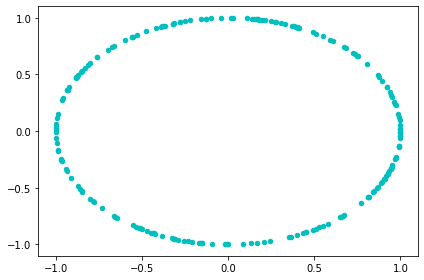
\includegraphics[width=0.4\textwidth]{circle_sampling.png}}
%     \subtop[Sphere samples      
%     \label{fig:sphere_sampling}]
%         {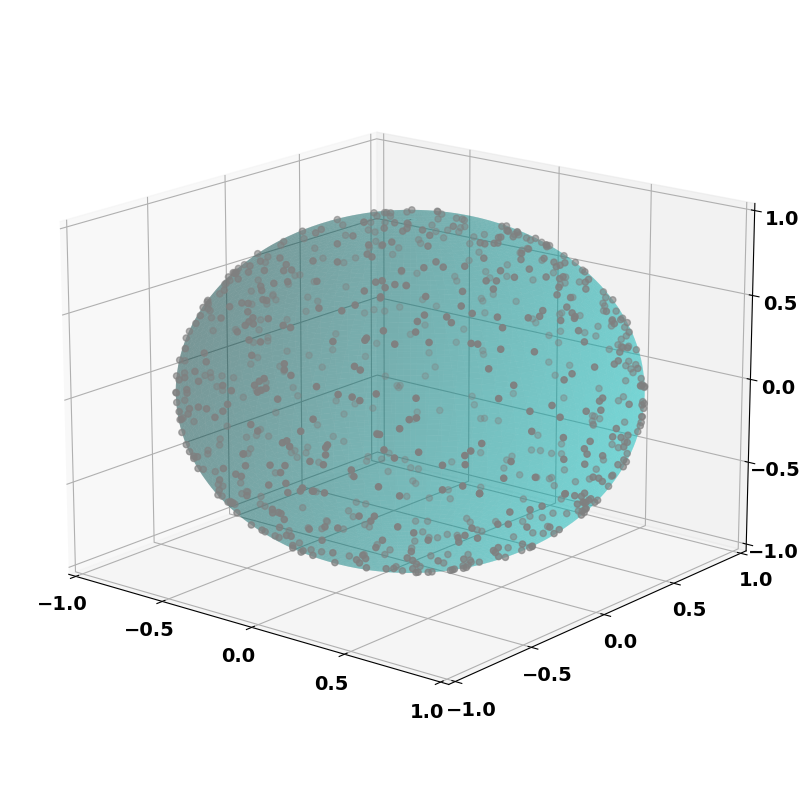
\includegraphics[width=0.4\textwidth]{sphere_sampling.png}}
%     \caption{Samples drawn from 1D and 2D manifold.}
% \end{figure}

One popular algorithm for calculating manifolds is diffusion maps \cite{diffusionMaps}, 
which is a non-linear approach for calculating low-dimensional manifolds
for (high-dimensional) datasets, using Graph Laplacian.
Vector diffusion maps \cite{vectorDiffusionMaps} generalize the concept of diffusion maps for vector fields.
Multi-frequency vector diffusion maps \cite{multiDiffusionMaps} 
can be seen as an extension to vector diffusion maps, which works well even on highly noisy environments.
\citet{cryoEmMutliDM} successfully applied multi-frequency vector diffusion Maps in cryo-EM setting,
 where it was used for denoising purpose.

\paragraph{Manifold assumption:}
\label{sec:manifoldAssumption}
Manifold assumption is a popular assumption for high-dimensional datasets.
For a given dataset in high-dimension, one can assume that data points are samples drawn from a low-dimensional manifold,
that embeds the high-dimensional space. 
Therefore, if underlying manifold can be approximated, a dimensionality reduction
is established as one can embed the data points in the low-dimensional manifold space.
There is a complete area of research devoted to this manifold assumption called Manifold Learning\cite{ManifoldLearning},
but it is not only used there.

\paragraph{Manifold calculation:}
Manifold of a dataset can be calculated the following:

\begin{enumerate}
    \item Construct k-NN graph from observations (see section~\ref{sec:graphConstruction}).
    \item Calculate the (normalized) Graph Laplacian.
    \item Extract the second, third (and fourth) smallest eigenvectors.
\end{enumerate}

Therefore, it can be observed how the manifold of classical tomography and cryo-EM objects look like.
In the following, the Shepp-Logan phantom (figure~\ref{fig:phantom}) is used as an example of classical tomography.
In figure~\ref{fig:phantom_sinogram}, figure~\ref{fig:phantom_sinogram_noisy} and figure~\ref{fig:phantom_sinogram_noisy_high} 
sinogram of the original phantom and phantoms, where gaussian noise was added, are shown.


\textbf{TODO: fix figures}
% \begin{figure}[H]
%     \centering
%     \subbottom[Shepp-Logan phantom          \label{fig:phantom}]{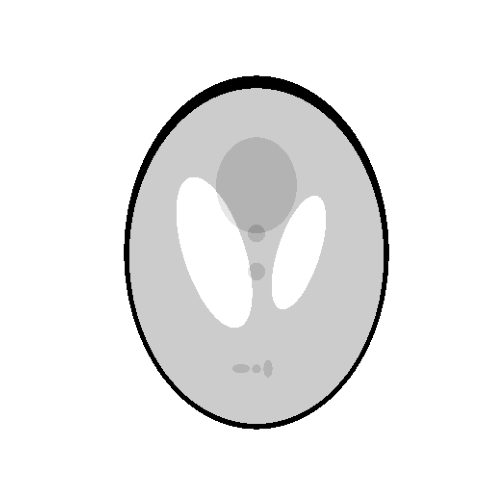
\includegraphics[width=0.18\textwidth]{phantom.png}}
%     \subbottom[Original sinogram            \label{fig:phantom_sinogram}]{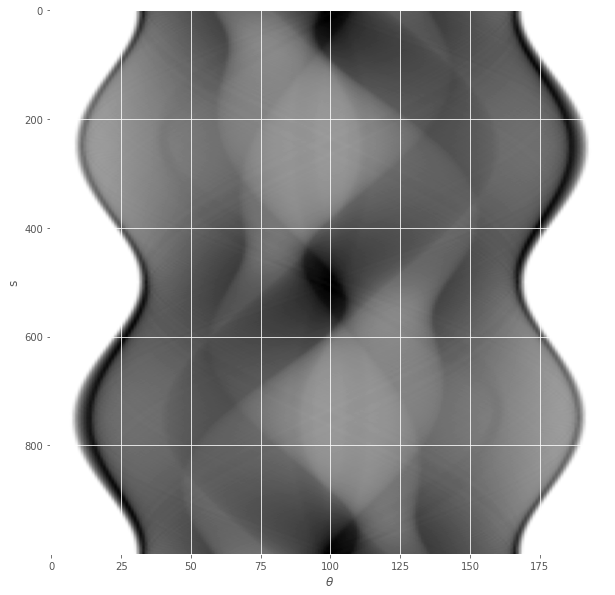
\includegraphics[width=0.18\textwidth]{phantom_sinogram.png}}
%     \subbottom[Noisy sinogram               \label{fig:phantom_sinogram_noisy}]{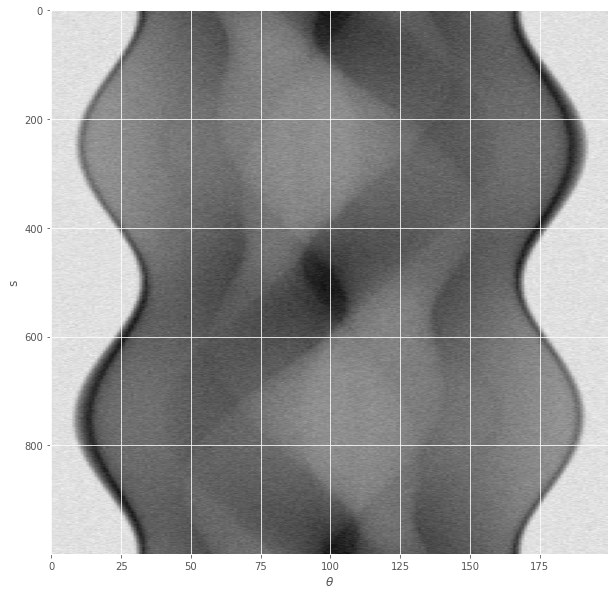
\includegraphics[width=0.18\textwidth]{phantom_sinogram_noisy.png}}
%     \subbottom[Highly noisy sinogram               \label{fig:phantom_sinogram_noisy_high}]{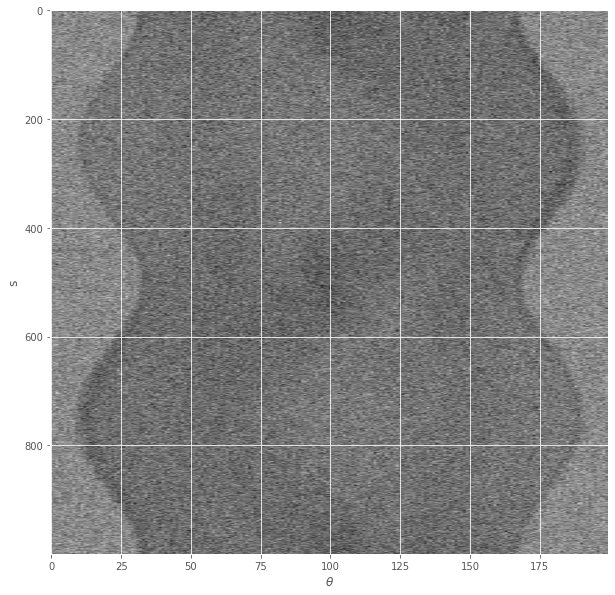
\includegraphics[width=0.18\textwidth]{phantom_sinogram_noisy_high.png}}
%     \caption{Shepp-Logan phantom and sinograms}
% \end{figure}

In Figure~\ref{fig:phantom_second_third_evec} the manifold calculated from original phantom Graph Laplacian
can be seen and it is a perfect circle. 
Further, in figure~\ref{fig:phantom_second_third_evec_noisy}
noisy version with $\sigma=2$ is plotted and the manifold is not a perfect circle, but circle like.

The more noise is added, the less manifold looks like a circle. In figure~\ref{fig:phantom_second_third_evec_noisy_high}
the manifold for $\sigma=100$ is plotted. In all plots, k-NN graphs have been constructed with $k=10$. 

\textbf{TODO: fix figures}
% \begin{figure}[H]
%     \centering
%     \subbottom[Original phantom manifold      \label{fig:phantom_second_third_evec}]{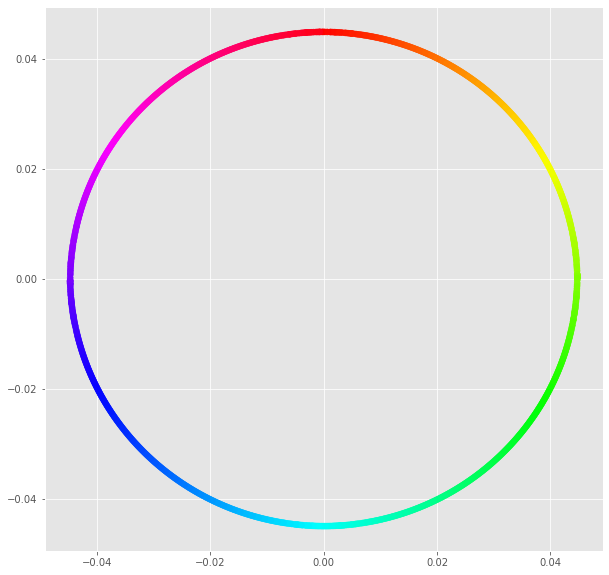
\includegraphics[width=0.25\textwidth]{phantom_second_third_evec.png}}
%     \subbottom[Noisy phantom manifold\label{fig:phantom_second_third_evec_noisy}]{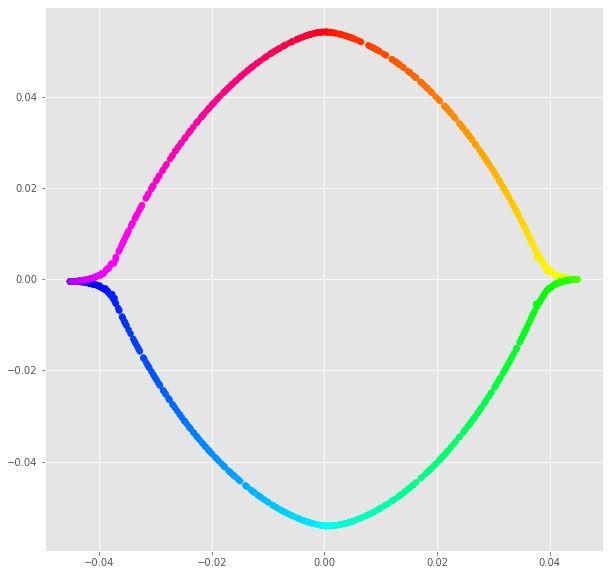
\includegraphics[width=0.25\textwidth]{phantom_second_third_evec_noisy.png}}
%     \subbottom[Highly-noisy phantom manifold \label{fig:phantom_second_third_evec_noisy_high}]{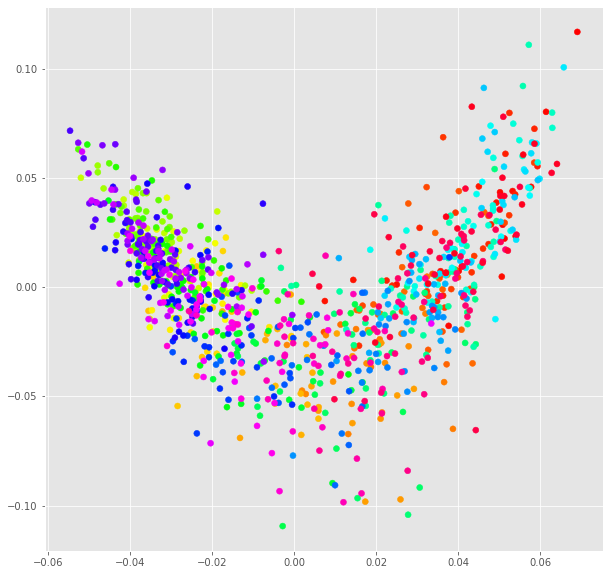
\includegraphics[width=0.25\textwidth]{phantom_second_third_evec_noisy_high.png}}
%     \caption{Shepp-Logan phantom manifolds}
% \end{figure}


\begin{tcolorbox}[colback=red!5!white,colframe=red!75!black]
    In the field of classical tomography and cryo-EM, the underlying low-dimensional manifold is well defined for none-noisy data.
    In the 2D case of classical tomography, the underlying manifold is a circle, whereas in 3D case of cryo-EM the manifold
    is defined as a sphere.
    This fact can be exploited during learning (e.g. by using Wasserstein loss function (see \ref{sec:wasserstein-metric})).
\end{tcolorbox}

\subsection{Connection to Machine Learning}

Graph Laplacian is used for dimensionality reduction for high-dimensional data, as well as spectral clustering and semi-supervised learning.
\citet{LaplaceRandomProjections} used Graph Laplacian in a complete other domain, namely in tomography. 
They showed that Graph Laplacian approximates the Laplace-Beltrami operator.
Further, Graph Laplacian is depended on the adjacency matrix $A$, if $A$ is noisy, Graph Laplacian will be noisy as well.

\subsection{Graph Deep Learning}
As already mentioned, Graph Denoising can be seen as a way of link predication. 
The state-of-the-art method for solving link prediction are \textit{Graph Deep Learning} approaches.
Graph Deep Learning is a fast evolving field in research. With Graph Neural Networks (GNN) \cite{GNN} the framework
for neural networks with graphs has been established. 

Using Graph Convolutional Networks (GCN) \cite{GCN} for graph feature extraction is a popular way. 
With GCN a new feature representation is iteratively learned for the node features (edge features are not considered).
It can be seen as an averaging of nodes over their neighbourhood where all neighbours get the same weight combined with some non-linear activation (e.g. ReLU). 
To consider the node itself in averaging they apply the so-called "Renormalization trick", where self-loops are added to the 
adjacency matrix and after every layer, a normalization step is applied. 
The topology of the graph will not be adjusted during  learning process.

\citet{GAT} extended the concept of GCN with attention and not all the neighbouring nodes get the same weight (attention).
Simple Graph Convolutional Network \cite{simpleGCN} proposed a simplified version of GCN.
They could verify their hypothesis that GCN is dominated by local averaging step and non-linear 
activation function between layers do not contribute to much to the success of GCN. 
Therefore, it can be seen as a way of power iteration (see \ref{sec:powerIterations} for further information) over the adjacency matrix with normalization in every layer.
\citet{dynamicGCN} proposed an extension to GCN by not operating on the same graph in every layer but adopting
underlying graph topology layer by layer.


\chapter{GAT-Denoiser}
\label{sec:contribution}

In this Chapter, I introduce my methodological approach.
As a result, a GNN is derived which is called \textit{GAT-Denoiser}.
Its main components and overall architecture is introduced.


\paragraph{Goal:}
CT and cryo-EM in the high-noise regime is the domain of interest.
For a given set of observations, a denoising model is sought, such that
it enables denoising of observations. As a first step towards an algorithm
which works for unknown observation angles, they are fixed during practical 
part of this Thesis.


\paragraph{Input graph:}
As $\theta$ is fixed, angle corresponding to each observation are known. 
Based on these angles, neighboring nodes can be connected, and a graph can be established.

\begin{tcolorbox}[colback=red!5!white,colframe=red!75!black]
  For GAT-Denoiser, this entails that graph topology is fixed and
  a k-NN graph can be constructed from $\theta$.
\end{tcolorbox}

\section{Pipeline}
\label{sec:concept}

In the following section, the GAT-Denoiser pipeline is introduced. 
The pipeline consists of three neural network parts, namely convolution, GAT and U-Net.
For readers who are not familiar with these concepts, Chapter~\ref{sec:neural_networks} present an introduction.

GAT-Denoiser is a GNN and has two main components, namely convolution layers and GAT layers.
The main idea of GAT-Denoiser is to enable denoising of observations:
\begin{equation}
  \textit{GAT-Denoiser} (\cdot) : L^2(\tilde{\Omega}) \to  L^2(\tilde{\Omega}) , y \mapsto \textit{GAT-Denoiser} (y) 
\end{equation}

% The GAT is expected to denoise observation signal with its neighbours by averaging. 
% Further, convolution is added to denoise single observations.

Input $y$ of GAT-Denoiser is a noisy observation and output is a denoised version.
GAT averages over observation neighbors and convolution denoise single observations. 
For every GAT layer there is a preceding convolution. 
In the case of CT, convolution is in 1D, where for cryo-EM it is in 2D.

\begin{tcolorbox}[colback=red!5!white,colframe=red!75!black]
  The GAT denoise observation signal with its neighbors by averaging. 
  Further, convolution is added to denoise single observations.
\end{tcolorbox}


But, the main overall goal is to get the best possible reconstruction 
from noisy observation $y$ which approximates original object $x$ and 
not just denoise observation $y$ which approximates noiseless observation $p$.


\begin{equation}
  \begin{aligned}
    x \approx   &\textit{Recon} \left( \textit{GAT-Denoiser} \left( y \right) \right), \\
    \text{with } &\textit{Recon} : \textit{UNet} \left( \textit{FBP} \left( \cdot \right) \right)  
  \end{aligned}
\end{equation}

Therefore, an end-to-end learning approach is used where quality of reconstruction is 
compared during GAT-Denoiser training, which is expected to perform better than 
only optimizing denoising of observations.

\textbf{TODO: remove header}
In Figure~\ref{fig:overall-concept} overall GAT-Denoiser pipeline is illustrated.

\begin{figure}[H]
  \centering
  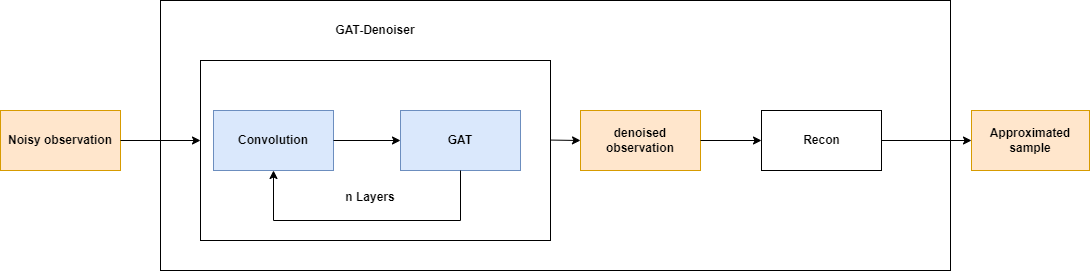
\includegraphics[width=\textwidth]{Overall_GAT-Denoiser_Pipeline.drawio.png}
  \caption{GAT-Denoiser pipeline}
  \label{fig:overall-concept}
\end{figure}

\textbf{TODO: link U-Net}


\section{Layers}
\textbf{TODO: rewrite chapter}
Therefore, input (noisy sinogram) will be in $\mathbb{R}^{N \times M}$ as well as output (denoised sinogram). 

In Figure~\ref{fig:architecture-detailed}, detailed GNN architecture can be seen.
It is parametrized with $channels$, $heads$ and $layers$. 
The number of channels in convolution can be increased with parameter $channels$.
Further, $heads$ determine the number of heads used in the GAT layers and parameter 
$layers$ defines how many convolution and GAT layers are stacked together.

\textbf{TODO: In figure everything bold! Replace parameters with c, h and l? Remove header}


\begin{figure}[H]
  \centering
  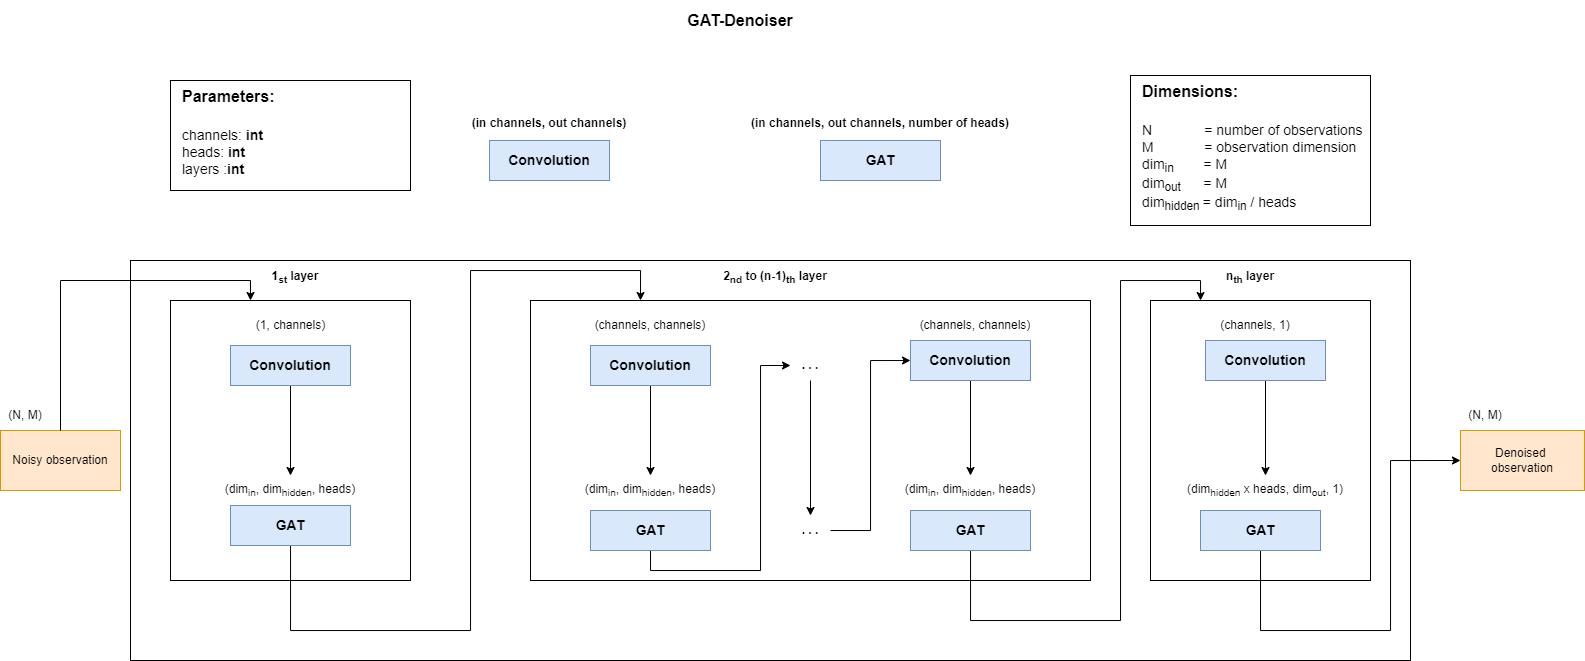
\includegraphics[width=\textwidth]{GAT_Architecture_Detail.drawio.png}
  \caption{Overall GAT-Denoiser architecture}
  \label{fig:architecture-detailed}
\end{figure}


For every layer, first convolution and then GAT is processed. 
Convolution in the whole network was defined with kernel size of 3 and padding 1,
therefore, dimension of convolved signal will not change. 
Convolution can be defined with different parameters, but output signal needs to have 
same dimension as input signal.
Further, additional convolutional channels can be used for learning.
If parameter $channels > 1$, channels are increased in the first convolution layer 
and decreased in the last one.
Parameter $heads$ controls multi-head approach for GAT. Input and hidden dimension
of GAT is $M$ if no heads are used.
If multi-head attention is used, hidden dimension will be set to $M / heads$.
In the last GAT layer, everything gets prepared for output dimension and 
averaging with 1 head is applied.



\paragraph{K-hop neighborhood:}
In GNNs, multiple layers expose the k-hop neighborhood. So for a network with $k$ layers,
network operates on the $k$-hop neighborhood. In GAT-Denoiser, this corresponds
to the layers of GAT. Therefore, if writing from one layer, it is referring to convolution and GAT together.

\section{Training}

\subsection{Loss}

\label{sec:contr_training}
An end-to-end learning approach is used where quality of reconstruction is 
compared in the loss.

Therefore, the outcome of GAT-Denoiser is not directly part of the loss, but first reconstruction will be computed.
Reconstructions can be nicely compared with the $\ell2$-norm:

\begin{equation}
  \label{eq:loss_reco}
  \mathcal{L} = \parallel x_i - \textit{Recon} ( \textit{GAT-Denoiser}(A(x_i, \theta, s) + \eta)) \parallel ^2_2
\end{equation}

As $x_i$ is part of the loss, access to original object is needed during training.

Further, U-Net will be jointly used with FBP as reconstruction. 
Thus, U-Net needs to be first pre-trained with the dataset.
One could also consider training U-Net and GAT-Denoiser jointly.

\textbf{TODO: Add Loss section with part from second loss.}


One could also consider computing loss from GAT-Denoiser output directly, therefore on denoised observation level.
For LoDoPaB-CT dataset, this would mean to compare clean sinogram with denoised sinogram:

\begin{equation}
  \label{eq:loss_sino}
  \mathcal{L}_{sino} = \parallel p_i - \textit{GAT-Denoiser}(A(x_i, \theta, s) + \eta) \parallel ^2_2
\end{equation}

%\chapter{Preliminaries and Problem Setup}
\label{sec:preliminariesProblem}


In the following chapter, the problem setup handled by the Master Thesis will be explained.
Further, preliminaries regarding assumptions and other decisions are defined.

\section{Tomographic reconstruction problem}
\label{sec:reconstructionProblemCT}
Tomographic reconstruction\cite{tomographicReconstruction} is a popular inverse problem \cite{tomographicReconstruction}. 
The aim is to reconstruct an object $x$ from its observed projections $\mathcal{P}=[\rho_0, \rho_1, \dots, \rho_N]$.
More formally, the aim is to recover some density function $f$ from overserved samples $y$, taken from the line-integral $\rho(\cdot)$.

The problem can be defined as a two-dimensional (2D) problem but also as a three-dimensional (3D) problem. 
In the following, we focus on the 2D case.
In 2D, also called classical tomography reconstruction problem, the underlying density function is in two dimensions and the measurement lines lie on a plane.

The problem automatically gets harder, if we deal with incomplete datasets (subset of measured lines, limited angle data) but also with noisy observations.

\paragraph{Classical tomography reconstruction}

First of all, lets define the line integral $\rho$ of our unknown density function $f$ in the classical case:

\begin{equation}
    \begin{aligned}
        y_i &= \rho_i (\theta_i, s_i)
        \rho(\theta, s)   &=  R f(\theta, s) \\
        R f(\theta, s) &=  \int_{-\infty}^{\infty} f(x(z), y(z)) dz \\
        &= \int_{-\infty}^{\infty} f((z \sin \theta + s \cos \theta), (-z \cos \theta + s \sin \theta)) dz \\
    \end{aligned}
\end{equation}

where $\rho$ is the line integral of the density function $f$, $\theta$ the projection angle and $s$ the distance from the origin.

In the 2D case, the line integral corresponds to the Radon-Transform $Rf$
With the 2D Radon transform, we can map the density function $f$ to the sinogram $\rho$. 

\paragraph{Filter Backprojection}
\label{sec:filterBackProjection}
Filter Backprojection (FBP) is a reconstruction method, typically used in classical tomography reconstruction.
It allows to solve for $\rho$ and is equivalent to the inverse of the Radon Transform
and is related to the Fourier transform. 

Basically, it maps sinograms of $\rho$ back to the density function $f$.

\begin{equation}
    f(x) = \int_{0}^{\pi} Rf(\theta, s) |_{s=x \cdot (- \sin \theta, cos \theta) } d \theta
\end{equation}

The disadvantage of the algorithm is, that it only works for complete data and without noise
and needs adjustments when dealing with such scenarios. 

\section{Cryo-EM}
Similar to tomographic reconstruction, there is the cryo-EM reconstruction problem\cite{cryoEmMath}.
It can be seen as a 3D reconstruction problem as the original object $x$ to be reconstructed is in 3D.

During observation process, the object will be frozen, which results in a random rotation, and from this intermediate state 
projections $\mathcal{P}=[\rho_0, \rho_1, \dots, \rho_N]$ are observed.

More formally, the aim is to recover some density function $f$ from overserved samples $y$, taken from 
randomly rotated, projected 2D samples.

The two problem are highly related, but the cryo-EM reconstruct is even harder than tomographic reconstruction.
During CT observation, the patient is asked to not move and therefore, the angles of projection is known, whereas
in cryo-EM this information will be lost during the freezing process.
Secondly, the high level of noise makes cryo-EM much more challenging regarding tomographic reconstruction.

\begin{equation}
    \label{eg:cryoEmSimple}
    y_i = \Pi_z \left( R_{\theta} x) \right) + noise,
\end{equation}

where $R_{\theta}$ is a 3D rotation and $\theta \in SO(3)$, $\Pi_z$ the tomographic projection.

\paragraph{Extended formula:} 
The equation~\ref{eg:cryoEmSimple} is a simplified version of the cryo-EM reconstruction problem.
First of all, the point spread function (PSF) of the microscope is not taken into account.
Moreover, due to structural variety in the molecule, the underlying object $x$ is not the same 
for every observation but can be seen as a random signal from an unknown distribution defined over all possible molecules structures.

The extended version can be defined as follows
\begin{equation}
    \label{eg:cryoEmExtended}
    y_i = h_i * \Pi_z \left( R_{\theta} x_i) \right) + noise,
\end{equation}

where $h_i$ is the PSF of the microscope and $*$ defines the convolution.

\section{General form}
\textbf{TODO:}
We don't observe $y_i \in L^2$ but $y_i = y_i(\Delta) $, with $\Delta \subset (R^{D-1})^N$ a grid containing $N$ points. 

As the tomographic reconstruction and the cryo-EM reconstruction are rather similar, 
the aim of the Master Thesis will be to design an algorithm, that can be applied in both scenarios.

Therefore, a general form of the two problem will be defined in the following.
First of all, we define $x \in L^2(\Omega)$, where $L^2$ is the Lebesgue space and $\Omega$
is the sample space $\Omega \subset \mathbb{R}^D$, where $D$ is the dimension of the sample space. 
Further we define $\tilde{\Omega} \subset \mathbb{R}^{D-1}$.


\begin{equation}
    \begin{aligned}
        y_i &= A(x, \theta) + \eta \\
    \end{aligned}
\end{equation}

where $y_i$ is the observed sample, $x$ our original object, $A$ a non-linear operator 
$A: x \in L^2(\Omega) \rightarrow \tilde{x} \in L^2(\tilde{\Omega})$ and $\eta ~ \mathcal{N}(O, \sigma^2 I)$ gaussian noise.

\paragraph{Classical tomography reconstruction:}

For classical tomography, the parameters can be defined with $D=2$ and $\theta \in SO(1)$.
Further, $A(\cdot)$ can be defined as the Radon transform. 
A distance measure between samples can be set up by using the l2-norm $\norm{y_i - y_j}$.

\paragraph{Cryo-Em reconstruction:}
For classical tomography, the parameters can be defined with $D=3$ and $\theta \in SO(3)$.
Further, $A(\cdot)$ can be defined as $\Pi_z \left( R_{\theta} x) \right)$ 
where $R_{\theta}$ is a 3D rotation and $\theta \in SO(3)$, $\Pi_z$ the tomographic projection.
As the samples are drawn with some random 3D rotation and then will be projected, it can 
happen that two samples are equivalent up to an 2D rotation. 
Consider a first example $y_1$, which has no 3D rotation at all and 
a second sample $y_2$ with a rotation only in in x-y plane by 45°.
The two samples have a defined in-plane rotation $g$, such that $g y_1 = y_2$.
Therefore, in our distance measure we add this term of in-plan rotation: $min_{g \in SO(1)}\norm{g * y_i - y_j}$, 
which is inspired by the work of \cite{multiDiffusionMaps}. 


\subsection{Manifold assumption}
In the reconstruct problem, we can apply the manifold assumption from section \ref{sec:manifoldAssumption}.
Moreover, in the none-noisy case, we can even assume how this manifold looks like.

The manifold, and therefore, a low-dimensional embedding, can be calculated the following:

\begin{enumerate}
    \item Construct the knn-graph from our observations (see section~\ref{sec:graphConstruction}).
    \item Calculate the normalized Graph Laplacian (see equation~\ref{eq:normalizedGraphLaplacian}).
    \item Extract the second, third (and fourth) smallest eigenvectors (see FSM section~\ref{sec:FoldedSpectrumMethod}).
\end{enumerate}

The manifold in the 2D case is a circle and in the 3D case, it will be a sphere.

\begin{figure}[H]
    \centering
    \subbottom[Shepp-Logan phantom          \label{fig:phantom}]{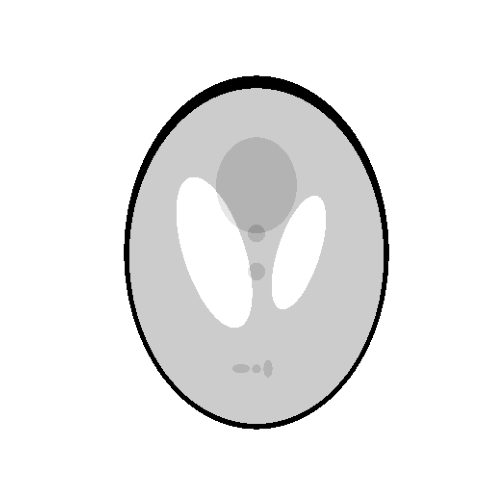
\includegraphics[width=0.18\textwidth]{phantom.png}}
    \subbottom[Original sinogram            \label{fig:ps:phantom_sinogram}]{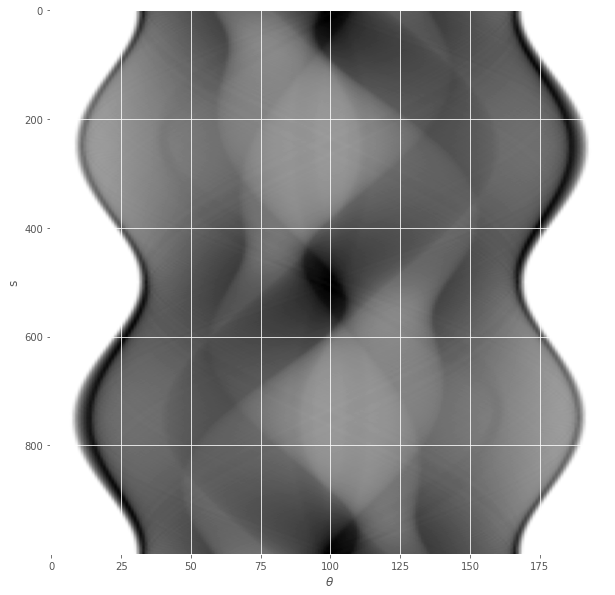
\includegraphics[width=0.18\textwidth]{phantom_sinogram.png}}
    \subbottom[Noisy sinogram               \label{fig:phantom_sinogram_noisy}]{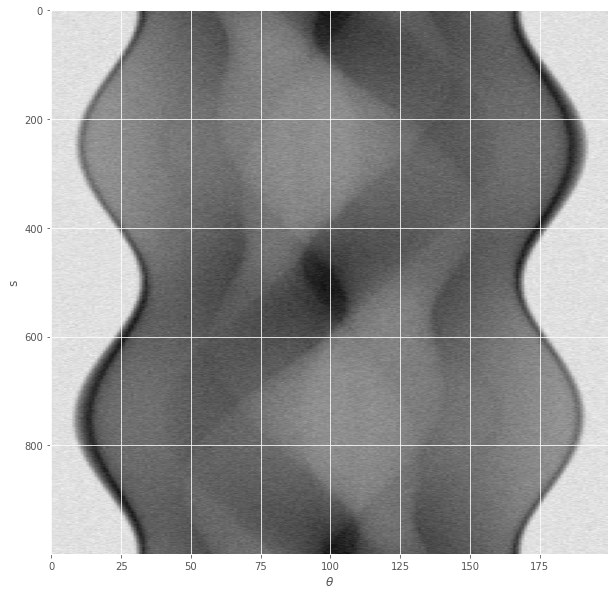
\includegraphics[width=0.18\textwidth]{phantom_sinogram_noisy.png}}
    \subbottom[2nd and 3rd smallest eigenvector of Graph Laplacian      \label{fig:phantom_second_third_evec}]{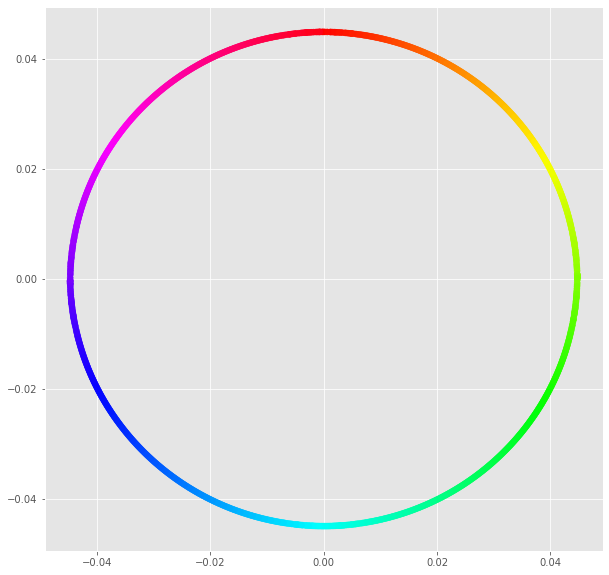
\includegraphics[width=0.18\textwidth]{phantom_second_third_evec.png}}
    \subbottom[2nd and 3rd smallest eigenvector of noisy Graph Laplacian\label{fig:phantom_second_third_evec_noisy}]{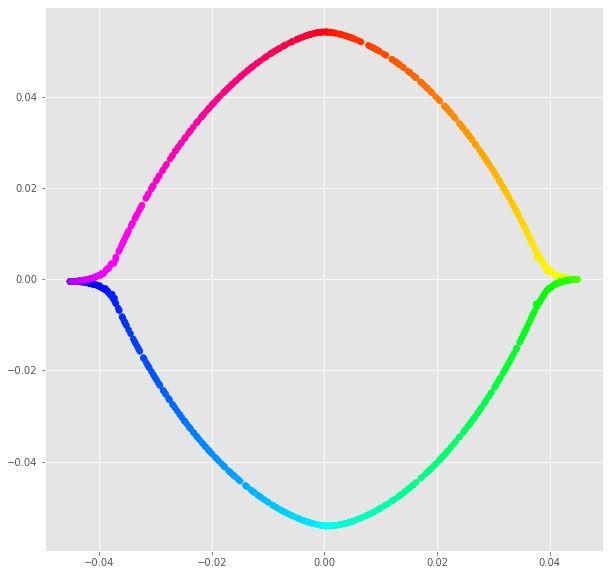
\includegraphics[width=0.18\textwidth]{phantom_second_third_evec_noisy.png}}
    \caption{Shepp-Logan phantom manifold}
\end{figure}

In Figure~\ref{fig:phantom_second_third_evec} the manifold calculated from the original Graph Laplacian
can be seen and it is a perfect circle. Next to it, in Figure~\ref{fig:phantom_second_third_evec_noisy}
the noisy version with $\sigma=2$ is plotted and the manifold is circle like but not at all like from the original one.

The more noise we add, the less the manifold looks like a circle. In Figure~\ref{fig:phantom_second_third_evec_noisy_high}
the manifold for $\sigma=100$ is plotted.

\begin{figure}[H]
    \centering
    \subtop[Highly noisy sinogram               \label{fig:phantom_sinogram_noisy_high}]{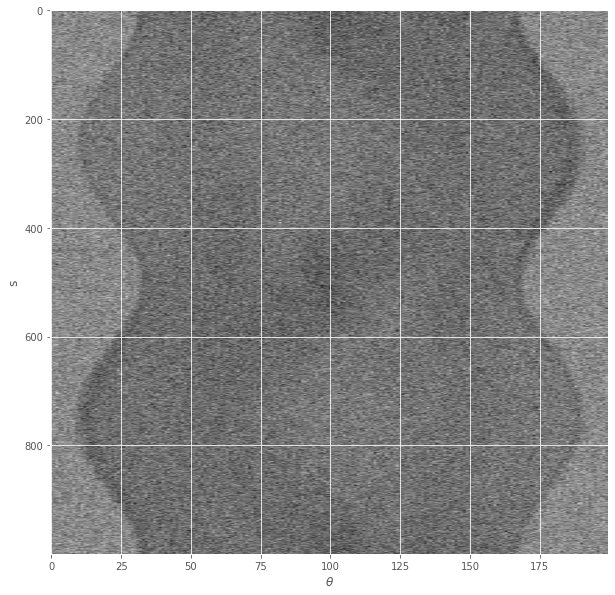
\includegraphics[width=0.4\textwidth]{phantom_sinogram_noisy_high.png}}
    \subtop[2nd and 3rd smallest eigenvector of Graph Laplacian      \label{fig:phantom_second_third_evec_noisy_high}]{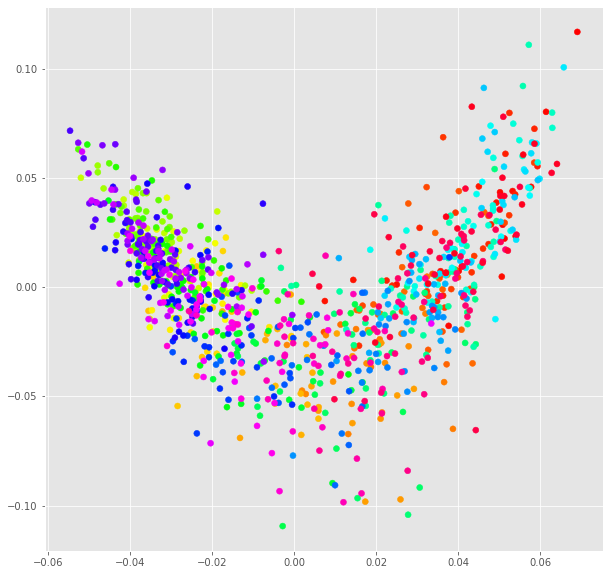
\includegraphics[width=0.4\textwidth]{phantom_second_third_evec_noisy_high.png}}
    \caption{Shepp-Logan phantom manifold for high noise level}
\end{figure}

In all the plots, knn-graph have been constructed with $k=10$. The showed example can be extended to 3D, where the underlying manifold corresponds to the sphere.
Again, the circle and sphere can be computed and for the none-noisy, the underlying manifold can be seen as known.


\section{Thesis problem}
During the Master Thesis, the reconstruction problem with unknown angles is considered. 
Moreover, the observed samples are considered to be noisy. 
The resulting proposed algorithm should work in the 2D and 3D scenario (classical tomography and cryo-Em).

The main idea is to exploit the fact, that the underlying manifold is known (circle in 2D and sphere in 3D). 
From our noisy observations, a manifold can be computed and compare it with the original manifold.
The comparison between the manifolds enables the possibility of a loss function and learning in general.

It is expected, that the folded spectrum \cite{foldedSpectrumMethod} introduced in section~\ref{sec:FoldedSpectrumMethod}
can be used to estimate the eigenvalues of the Graph Laplacian.
Further, as already mentioned in section~\ref{sec:wasserstein-metric}, the wasserstein metric is a good choice
as a loss function when it comes to dealing with data from a manifold distribution \cite{wassersteinGAN}, as in our case. 

The problem can be seen as Graph Denoising as observations are noisy and therefore, the proposed algorithm 
will denoise the graph based on the manifold assumption. 


\paragraph{Evaluation:}
During evaluation, 2D and 3D scenario will be considered. A first evaluation will be done on artificial constructed
toy-dataset. If time allows, real dataset from classical tomography and/or cryo-EM\footnote{https://www.ebi.ac.uk/emdb/} can be evaluated as well.
During evaluation, two baselines are considered which already solved the problem. The first one is a multi-frequency diffusion 
map approach\cite{multiDiffusionMaps, cryoEmMutliDM}, which aims to denoise cryo-EM images. 
Secondly, \cite{LaplaceRandomProjections} a Graph Laplacian approach solving classical tomography with random projection angles will be compare against.
The evaluation process is a first broad idea. Any adjustments in baseline papers or dataset are possible during 
the Master Thesis. The baseline papers are further addressed in the related work chapter~\ref{sec:relatedWork}
and detailed work packages are defined in chapter~\ref{sec:projectPlan}

%\chapter{Related Work}
\label{sec:relatedWork}

In the following section, related work will be introduced.


\section{Graph Deep Learning}
Graph deep learning is a fast evolving field in research. With Graph Neural Networks (GNN)

\cite{GNN}
\cite{GAT}

\subsection{Graph feature extraction with GCN}

\subsection{Graph Convolutional Network}
Graph Convolutional Networks (GCN) \cite{GCN} can be used for many tasks in the field 
of Graph Learning, such as node classification or link prediction. 
Basically, with GCN, a new feature representation is iteratively learned for the node features.

The basic concept is as follows:
For a given graph $G = \langle V,E \rangle$, with node features $X^{N x D}$ and adjacency Matrix $A$
where $N$ denotes the number of nodes and $D$ the number of node input attributes,

a novel node representation $Z^{N x F}$ will be learned, where $F$ is the number of output features.

$Z$ will be learned within a neural network, and every layer can be written by the following, non-linear function:

\begin{equation}
    \begin{aligned}
        H^{l + 1} &= f( H^l, A), \\
        \text{with } H^0 &= X , \\
        H^L &= Z, 
    \end{aligned}
\end{equation}

where $L$ is the number of layers in the neural network.
The model only differ in the choice of $f(\cdot,\cdot)$.

We are ready to define our first GCN. To keep it simple, $f(\cdot,\cdot)$ will be defined as the following:
\begin{equation}
    f( H^l, A) = \sigma (A H^l W^l)
\end{equation} 

Where $\sigma ( \cdot )$ is a non-linear activation function, such as ReLU and $W^l$ is
a weight Matrix of the layer $l$ of the neural network. As \citet{GCN} could show during experiments,
this choice of $f(\cdot,\cdot)$ is already very powerful and leads to state-of-the-art results.

\subsubsection{Renormalization trick}

With this model, we do have two problems and need to refine it further.
First of all, with the multiplication of $A$, we average over the neighbour nodes but
will ignore the node itself. Therefore, self-loops will be added to $A$.
The second problem is, that A is not normalized and if therefore, when multiplying with $A$,
the features of the nodes will change it scale. Therefore, we need to normalize $A$
such that all rows sum to one. This can be done with a simple multiplication with the D.

These two steps are called the Renormalization trick\cite{GCN}.
First of all, we can simple add the self-loops by adding the Identity Matrix to $A$, 
$\hat{A} = A + I$ and $\hat{D}$ is the degree Matrix of $\hat{A}$.
Now, we can achieve a symmetric normalization by multiplying $D^{-\frac{1}{2}} A D^{-\frac{1}{2}}$.

And finally, we can put all things together, and replace $A$ in the original equation:
\begin{equation}
    f( H^l, A) = \sigma (\hat{D}^{-\frac{1}{2}} \hat{A} \hat{D}^{-\frac{1}{2}} H^l W^l)
\end{equation} 


\subsubsection{Simple Graph Convolutional Network}
\textbf{Basically Power method with normalization}

Simple Graph Convolutional Network (SGC) \cite{simpleGCN} proposed a simplified version of GCN.
They could verify their hypothesis, that GCN is dominated by the local averaging step and the non-linear 
activation function between layers do not contribute to much to the success of GCN.

This makes the calculation simpler. We denote $S = \hat{D}^{-\frac{1}{2}} \hat{A} \hat{D}^{-\frac{1}{2}} $
and can use the fact that in every layer of the neural network, the same computation will take place.

\begin{equation}
    \begin{aligned}
        Z = S \dots S X W^1 W^2 \dots W^L \\
        Z = S^L X W^1 W^2 \dots W^L \\
        Z = S^L X W    
    \end{aligned}
\end{equation}

where $W$ is the matrix of all vector weights.



\subsubsection{Link to Graph Laplacian:}

In the section, we will have a look at the connection between SGC and Graph Laplacian.

We can define $x \in R^n$ as our signals and define the Fourier transform as $\hat{x} = U^T x$
and the inverse as $x = U\hat{x}$. 
With the transform, we can easily switch between spatial and Fourier(spectral) domain.

Further, we can define the graph convolution operation between signal $x$ and filter $g$.

\begin{equation}
    g \star x = U((U^T g) (U^T x)) = U \hat{G} U^T x,
\end{equation}

where $\hat{G}$ is a diagonal matrix where the elements are the 
spectral filter coefficients (eigenvalues?)

The graph convolution can be approximated by the $k$-th order polynomials of Laplacians:

\begin{equation}
    \approx \sum_{i=0}^{k} \Delta^i x = U \left ( \sum_{i=0}^{k}  \Theta_i \Lambda^i \right ) U^T x,
\end{equation}

where $\Delta = D - A$ and $\Theta_i$ are 
filter coefficients which correspond to polynomials of the Laplacian eigenvalues,
 $\hat{G} = \sum_i \Theta_i \Lambda^i$


 In the original \cite{GCN} paper, the approximation is done with $k = 1$ 
 \begin{equation}
     g \star x = \Theta (I + D^{-\frac{1}{2}} A D^{-\frac{1}{2}} )x,
 \end{equation}

, where \citet{GCN} further applies the renormalization trick, ending up replacing
$I + D^{-\frac{1}{2}} A D^{-\frac{1}{2}}$ with $\hat{D}^{-\frac{1}{2}} \hat{A} \hat{D}^{-\frac{1}{2}}$.

$I + D^{-\frac{1}{2}} A D^{-\frac{1}{2}}$ is also called first-order Chebyshev filter.

%\footnote{https://towardsdatascience.com/spectral-graph-convolution-explained-and-implemented-step-by-step-2e495b57f801}

%not read currently:
%\footnote{https://towardsdatascience.com/tutorial-on-graph-neural-networks-for-computer-vision-and-beyond-part-2-be6d71d70f49}




\cite{GCN}
\cite{simpleGCN}
\cite{dynamicGCN}



\section{Manifold Learning}
\cite{isomap}
\cite{LLE}
\cite{LaplacianEigenmaps}

\section{Random Walk approaches}

\cite{diffusionMaps}
\cite{vectorDiffusionMaps}
\cite{multiDiffusionMaps}


\section{Denoising}

\subsection{Image Denoising}

\subsubsection{Non local means}
Non local means is a state-of-the-art image denoising method \cite{noneLocalMean}.
In the name of the method are two important concepts, namely the \textit{mean}
and \textit{non local}.

For a given noisy image $v$, the denoised image is defined as:
\begin{equation}
    NL[v](i) = \sum{w(i,j) \; v(j)}
\end{equation}

where $w(i,j)$ is the weight between pixel $i$ and $j$ and fulfils two conditions:
\begin{itemize}
    \item $0 \le w(i,j) \le 1$
    \item $\sum_j{w(i,j) = 1}$
\end{itemize}

The weight can be seen as a similarity measure of the two pixels.
Moreover, these similarities are calculated over square neighbourhoods of the two pixels,
where the l2 norm of the neighbourhood is used.
Similar pixel neighbourhoods have a large weight and different neighbourhoods have a small weight.

More general, the denoised image pixel $i$ is computed as an weighted average of all pixels in the 
image, therefore, in a non local way.
Image Denoising
Graph Denoising

\subsection{Graph Denoising}

\cite{noneLocalMean}
\cite{learningToDrop}


\subsection{cryo-EM calcuation}

\section{Graph Laplacian Tomography From Unknown Random Projections}

\citet{LaplaceRandomProjections} introduces a Laplacian-based algorithm, with which 
reconstruction of a planar object from projects at random unknown directions is possible.

Overall, in computerized tomography (CT), reconstruction of an object with only samples of its projections
is a standard problem. In \citet{LaplaceRandomProjections} the problem was extended by the fact,
that the projection angle to the object is unknown.

Formally:
Given $N$ projection vectors $( P_{\theta_i}(t_1), P_{\theta_i}(t_2), \dots, P_{\theta_i}(t_N)$ 
at unknown angles $\{\Theta_i\}^N_{i=1}$ which are drawn from the uniform distribution of $[0, 2\pi]$
and $t_1, t_2, \dots, t_n$ are fixed n points (all equally spaced due to uniform distribution) 
find the underlying density function $\rho (x,y)$ of the object.

\subsection{Radon transform}

The radon transform $P_{\Theta}(t)$ is the line integral of $\rho$
along parallel lines $L$ at angle $\Theta$ and distance $t$ from the orign.

\begin{equation}
    \begin{aligned}
        P_{\Theta}(t) &= \int_L \rho (x,y) ds \\
                      &=  \int_{-\infty}^{\infty} \rho (x,y) \; \delta(x \cos \Theta + y \sin \Theta - t) dx \; dy
    \end{aligned}
\end{equation}

An algorithm for estimating angles from given projections have been introduced by \cite{formerUnkownRandomProjections}.
The introduced algorithm consists of three steps:
\begin{enumerate}
    \item Angle estimation
    \item Angle Ordering
    \item Joint maximum likelihood refinement of angles and shifts
\end{enumerate}

Step 2 was implemented by some nearest neighbour algorithm. In the work of 
\cite{LaplaceRandomProjections}, they introduced a new way of ordering the angles,
using Graph Laplacian.


\subsection{Laplace-Beltrami operator}
\cite{LaplaceRandomProjections} could show, that the graph Laplacian
 approximates the Laplace-Beltrami operator, if data points are uniformly distributed 
 over the manifold.

 Further, they showed that in the case of non-uniformly distributed data points, the Laplacian
 approximated the backward Fokker-Planck operator (which is a generalization of the Laplace-Beltrami operator).
 With that, at least the ordering of the angles can be estimated.

 Finally, with a small normalization of the Laplacian, the Laplace-Beltrami operator can also be 
 approximated in the non-uniform distributed case.

\subsection{Algorithm}

For a given set of projections vector $x_i = ( P_{\Theta_i}(t_1), \dots, P_{\Theta_i}(t_n))$ for $i = 1,2, \dots, mN$

The algorithm proposed in \cite{LaplaceRandomProjections} consists of five steps:

\begin{enumerate}
    \item Double the number of projections to 2mN (due to the fact that projections are symmetric)
    \item Construct the co-called density invariant Graph Laplacian $\tilde{L}$
    \item Compute $\theta_1(i)$ and $\theta_2(i)$ the first two nontrivial eigenvector of $\tilde{L}$
    \item Sort $x_i$ according to $\phi_i = \tan^{-1}(\theta_1(i) \; / \;\theta_2(i))$
    \item Reconstruct image using the sorted projections and estimated angles.
\end{enumerate}

Where $\tilde{L}$ can be constructed by the following way:

\begin{equation}
    \begin{aligned}
        W_{ij} = k \left ( \frac{\left \| x_i - x_j \right \|^2}{2 \epsilon}  \right ), \\
        i, j = 1, \dots, N
    \end{aligned}
\end{equation}

where $||\cdot ||$ is the euclidean-norm, $k$ a semi-positive kernel 
and  $\epsilon > 0$ the bandwidth of the kernel. As mentioned in \cite{LaplaceRandomProjections},
the kernel $k(x) = \exp (-x)$ is a popular choice.

With the newly computed weight Matrix $W$ and the degree Matrix $D$ corresponding to $W$, we can finally 
define $\tilde{L}$.

\begin{equation}
    \begin{aligned}
        \tilde{W} &= D^{-1} W D^{-1} \\
        \tilde{D} &= \text{Degree matrix corresponding to } \tilde{W} \\
        \tilde{L} &= \tilde{D}^{-1} \tilde{W} - I \\
    \end{aligned}
\end{equation}


\chapter{Evaluation}
\label{sec:evaluation}


Create artificial data to test algortihm
and add hand crafted noise.

Use CT tomography for simple 2D tomography case.
Shepp-Logan phantom.

Long view, application to cryoEM, 
but probably not possible during MS Thesis.

Baseline Papers

Multifrequency Vector diffusion maps \cite{multiDiffusionMaps}

and \cite{LaplaceRandomProjections}
\chapter{Conclusion & Discussion}
\label{sec:Conclusion}
Connect to 3D


%% ----------------------------------------------------------------
%\thesisappendix
\thesisbib
% \addtocontents{toc}{\protect\setcounter{tocdepth}{0}}
\begin{appendices}
	

\chapter{Mathematical Tools}
Some mathematical tools will be introduced in the following chapter.

\section{3D Rotation Matrix}
\label{app:3DrotationMatrix}
A rotation matrix is a transformation matrix used to perform rotations.
In the 3D case, matrix for rotating one single axis can be described as:
\begin{equation}
    R_{e_x} (\theta)
    \begin{bmatrix}
        1 & 0 & 0\\
        0 & \cos \theta & - \sin \theta \\
        0 & \sin \theta & cos \theta \\
    \end{bmatrix}
\end{equation}

\begin{equation}
    R_{e_y} (\theta)
    \begin{bmatrix}
        \cos \theta & 0 & \sin \theta\\
        0 & 1 & 0 \\
        - \sin \theta & 0 & cos \theta \\
    \end{bmatrix}
\end{equation}

\begin{equation}
    R_{e_z} (\theta)
    \begin{bmatrix}
        \cos \theta & - \sin \theta\\
        \sin \theta & \cos \theta & 0 \\
        0 & 0 & 1 \\
    \end{bmatrix}
\end{equation}

Where $e_x, e_y, e_z$ corresponds to the axis unit-vector (for x: $(1,0,0)$, etc.) and $\theta \in \mathbb{R}$.
To combine the single axis rotations, matrices can be multiplied with each other:

\begin{equation}
    \label{eq:3d-rotation}
    R (\theta) = R_{e_x} (\theta) R_{e_y} (\theta) R_{e_z} (\theta)
\end{equation}

In Equation~\ref{eq:3d-rotation}, angle $\theta$ is the same for all axis, which does not have to be.


\section{Power Iterations}
\label{sec:powerIterations}

Power iteration, also called power method, is an iterative algorithm
that approximates the largest eigenvalue of a diagonalizable matrix $A$.

The algorithm starts with a random vector $b_0$ or an approximation of the dominant eigenvector.

\begin{equation}
    \label{eq:powerIterations}
    b_{k+1} = \frac{Ab_k}{||Ab_k||}
\end{equation}

It will not necessarily converge. It only converges if $A$ has an eigenvalue strictly grater than its other eigenvalues
and initial vector $b_0$ is not orthogonal to the eigenvector associated with the largest eigenvalue.
 
  \chapter{Graph Laplacian Embedding}


\section{Manifolds}
\label{sec:manifolds}

\textbf{TODO:
it maps Rd to RD, if d<D. 
In our case, it map an angle in S1 (subset of R) to something in RM. The circle S1, is 1 dimensional, 
it depends only on 1 parameter, and can be represented in R2 like you did. 
I thinks (not 100 of sure of that right now) that the  rotation group is a manifold, 
it maps 1d parameter (rotation angle) to some rotation operator (which is high dimensional)
we don't calculate manifold. 
Diffusion maps (or graph Laplacian embedding) are a way to map high dimensional dataset to low dimensional one. 
When the data points are sampled from a manifold, the GL embedding is closely related to the manifold itself.
We can expect the GL embedding to share property of the original manifold, such as preservation of distances between points}


For high-dimensional data Euclidean distances are not meaningful
in the sense that they will not capture similar data points well. 
GL can be used to compute a low-dimensional embedding which can map from high-dimensional space to low-dimensional one.
In low-dimensional space, Euclidean distances make sense again. 

The manifold assumption is a popular assumption for high-dimensional datasets.
For a given dataset in high-dimension, one can assume that data points are samples drawn from a low-dimensional manifold,
that embeds the high-dimensional space. 
Therefore, if underlying manifold can be approximated, a dimensionality reduction
is established as one can embed data points in the low-dimensional manifold space.
There is a complete area of research devoted to this manifold assumption called Manifold Learning\cite{ManifoldLearning}.

\paragraph{Definition:}
Let manifold $M$ be defined as $\mathcal{M} = \{ f(x), f \in C^K, f: \mathbb{R}^D \to \mathbb{R}^d \}$.
Manifolds are a well established mathematical concept. In this Thesis, only 
$C^k$ differentiable d-dimensional manifolds defined by $\mathcal{M}$ are considered. 
When $d \ll D$, manifolds define a \textit{low-dimensional embedding}, which maps from high-dimensional space 
$\mathbb{R}^D$ to low-dimensional space $\mathbb{R}^d$.

Let's give two popular examples of manifolds, namely the \textit{circle} and the \textit{sphere}.
The circle is a 1D manifold, where $d=1$ and $D=2$. A sphere is a 2D manifold with $d=2$ and $D=3$.
In Figure~\ref{fig:circle_sampling}, 200 samples are drawn from a uniform distribution of the unit-circle manifold
and in Figure~\ref{fig:sphere_sampling}, 800 samples are drawn from a uniform distribution of the unit-sphere manifold,
as well as the sphere itself.

\begin{figure}[H]
    \hfill
    \subbottom[
        \label{fig:circle_sampling}]
        {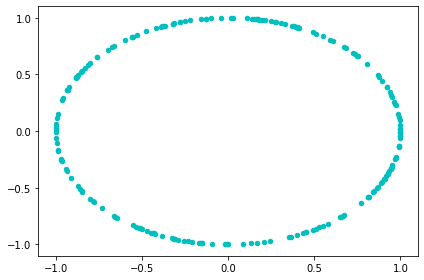
\includegraphics[width=0.4\textwidth]{circle_sampling.png}}
    \hfill
        \subbottom[      
    \label{fig:sphere_sampling}]
        {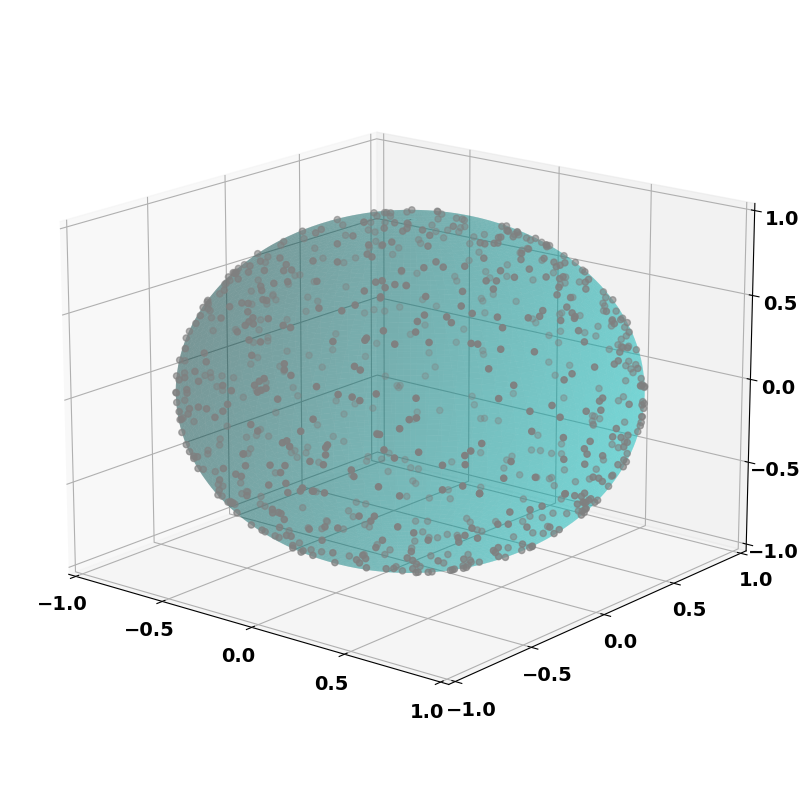
\includegraphics[width=0.42\textwidth]{sphere_sampling.png}}
    \hfill
        \caption{Samples drawn from 1D and 2D manifold: 
    \ref{fig:circle_sampling} circle samples,
    \ref{fig:sphere_sampling} sphere samples}
\end{figure}


\paragraph{GL-manifold}
\label{sec:manifold_calculation}
A simple low-dimensional embedding of a dataset can be computed with Graph-Laplacian by the following:

\begin{enumerate}
    \item Construct k-NN graph from observations.
    \item Calculate the (normalized) Graph Laplacian (see Equation~\ref{eq:gl}).
    \item Extract the second, third (and fourth) the smallest eigenvectors.
\end{enumerate}


Another popular algorithm for calculating a low-dimensional embedding is diffusion maps~\cite{diffusionMaps}, 
which is a non-linear approach using Graph Laplacian.
Vector diffusion maps~\cite{vectorDiffusionMaps} generalize the concept of diffusion maps for vector fields.
Multi-frequency vector diffusion maps~\cite{multiDiffusionMaps} 
can be seen as an extension to vector diffusion maps, which works well even on highly noisy environments.
\citet{cryoEmMutliDM} successfully applied multi-frequency vector diffusion Maps in cryo-EM setting,
 where it was used for denoising observations.


\subsection{Embedding quality}
\label{sec:embedding_quality}

Finding a good embedding, which approximates the  GL-manifold, is not easy and in our case, the embedding is dependent on $k$ during graph construction
as well as parameter $\theta$, $s$ and $\eta$ for obtaining observations.

K is an important parameter for building up a graph. If set too low, neighbors
do not capture similar data well as too few nodes are connected. 
Further, if k is set too high, strength of a neighbor 
is weakened and data is not well explained.
In Figure~\ref{fig:clean_manifolds}, GL-manifold computed by clean sinogram and k from 2 to 10 is illustrated.
One can see, that from $k \leq 4$ GL-manifold results in a perfect circle and with $k >  4$ is moves 
further away from the circle. 


\begin{figure}[H]
    \captionsetup[subfigure]{justification=centering}
    \centering
    \begin{subfigure}[t]{0.45\textwidth}
        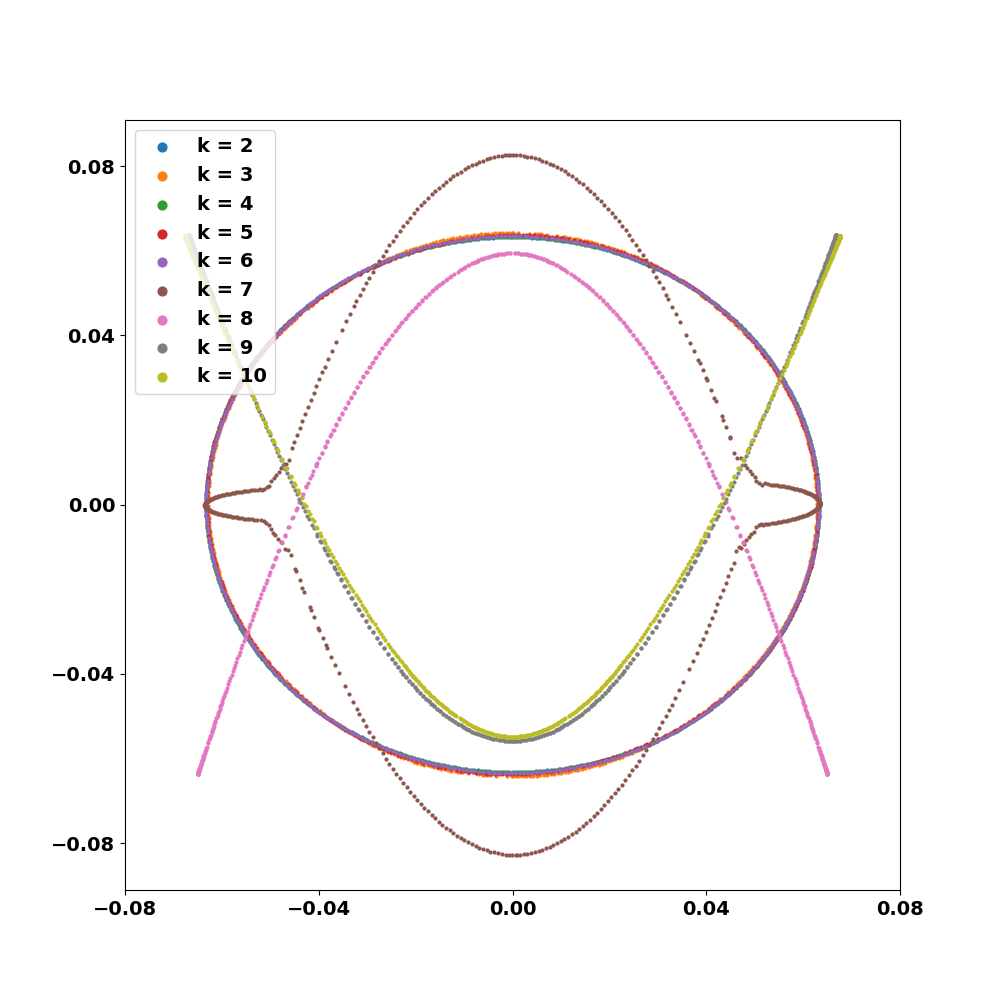
\includegraphics[width=\textwidth]{phaton_clean_manifold_kdifferent.png}
        \caption{Clean sinogram GL embeddings for different $k$.}
        \label{fig:clean_manifolds}
    \end{subfigure}\hfill
    \begin{subfigure}[t]{0.45\textwidth}
      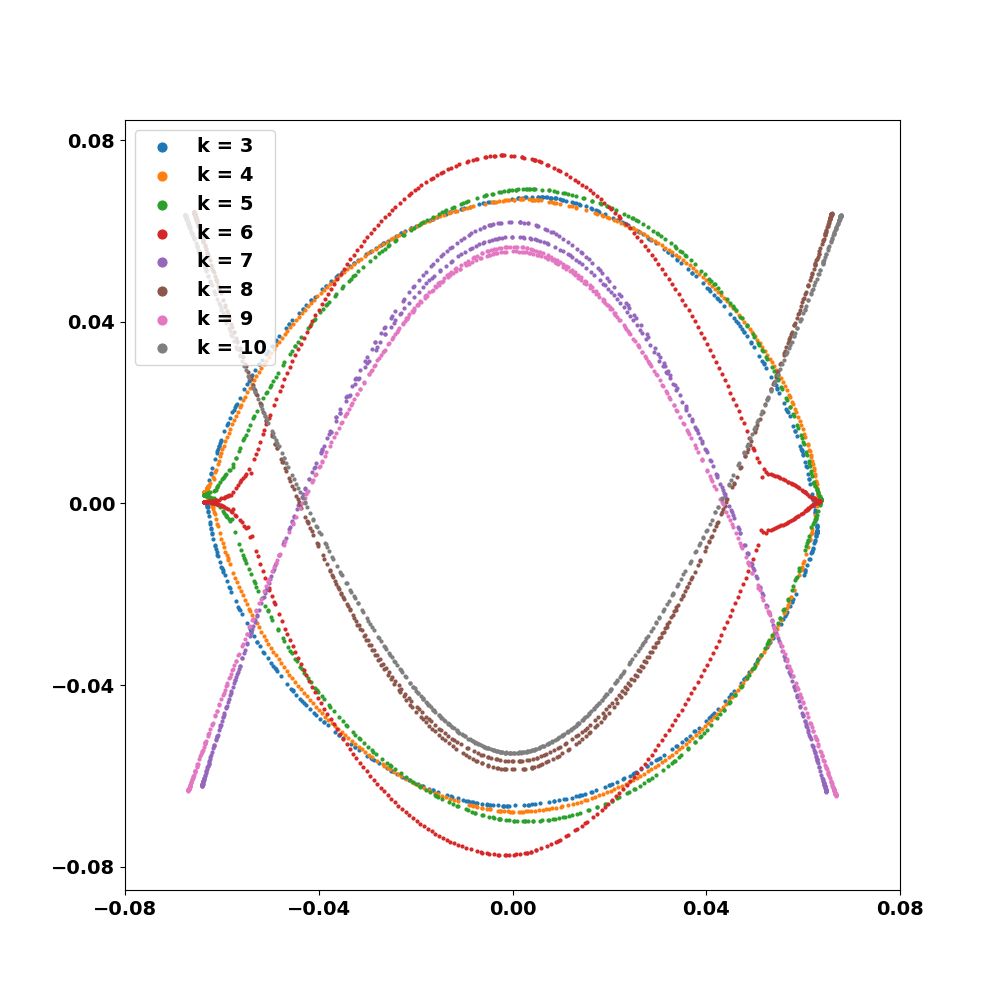
\includegraphics[width=\textwidth]{phaton_noisy_manifold_kdifferent.png}
      \caption{Noisy sinogram GL embeddings for different $k$.}
      \label{fig:noisy_manifolds}
    \end{subfigure}\hfill
    \caption{Shepp-Logan phantom sinogram GL eigenvectors}
  \end{figure}

If data is noisy, it is expected to be harder to construct a meaningful GL-manifold, as some connections within
the graph will be noisy. This is exactly what is illustrated in Figure~\ref{fig:clean_manifolds}, where 
different GL-manifold for noisy sinogram (SNR=20dB) and k from 3 to 10 are illustrated.
GL-manifold can never express data with a perfect circle. As noise is chosen rather moderate, GL-manifold has still some 
power to express underlying data and is expected to decrease, if noise is increased.


Further, when observing a sinogram, $\theta$ defines how many observations (straight lines) are drawn
and $dim(s)$ defines the amount of sampling points. Both have great impact to expressiveness of our sinogram.
In Figure~\ref{fig:clean_manifold_200} GL-manifold with $\theta \in \mathbb{R}^{200}$ and k=6 is illustrated
for clean sinogram. It looks like 6 are too many neighbors, as the perfect circle cannot be established anymore.
But, if $\theta$ is increased $\theta \in \mathbb{R}^{500}$, more nodes are available to choose good neighbors from
and a perfect circle can be established (figure~\ref{fig:clean_manifold_500}).

\begin{figure}[H]
    \captionsetup[subfigure]{justification=centering}
    \centering
    \begin{subfigure}[t]{0.45\textwidth}
        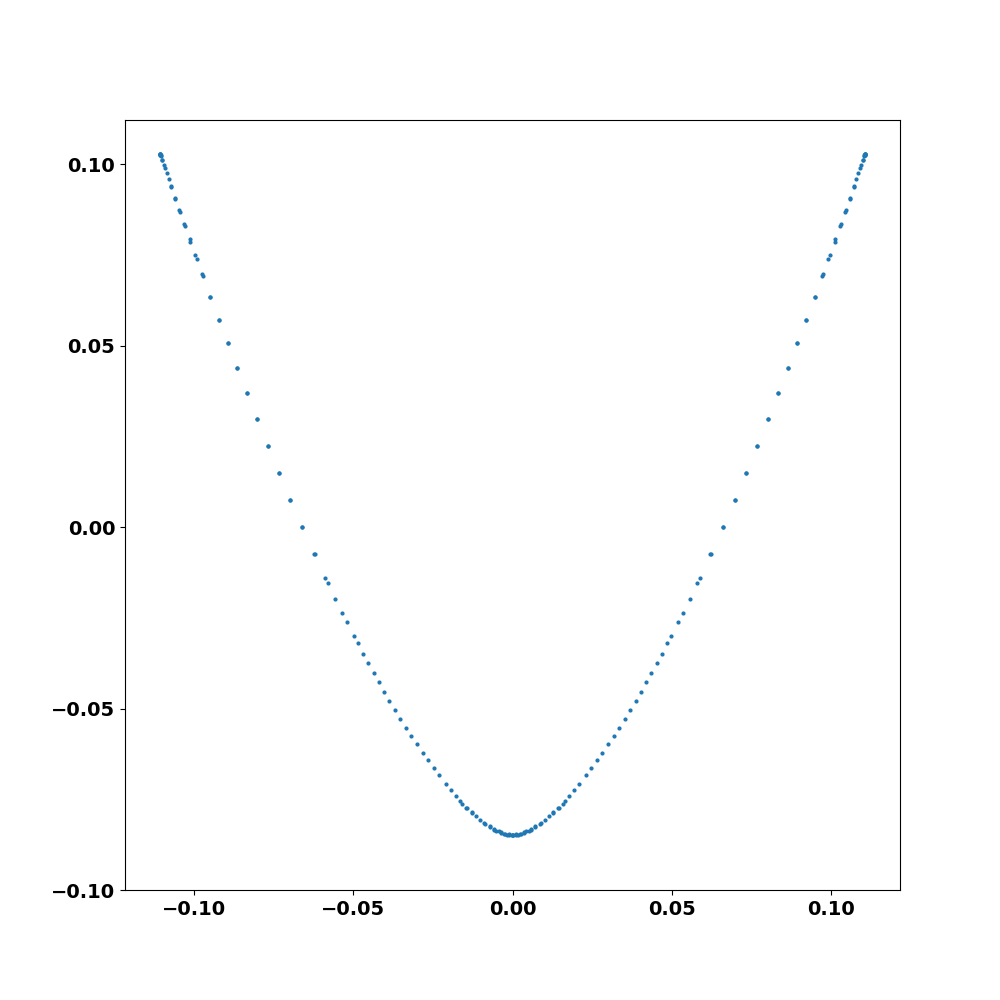
\includegraphics[width=\textwidth]{phaton_clean_manifold_200_k6.png}
        \caption{Clean sinogram GL-manifold, $k = 6$ and 200 samples}
        \label{fig:clean_manifold_200}
    \end{subfigure}\hfill
    \begin{subfigure}[t]{0.45\textwidth}
      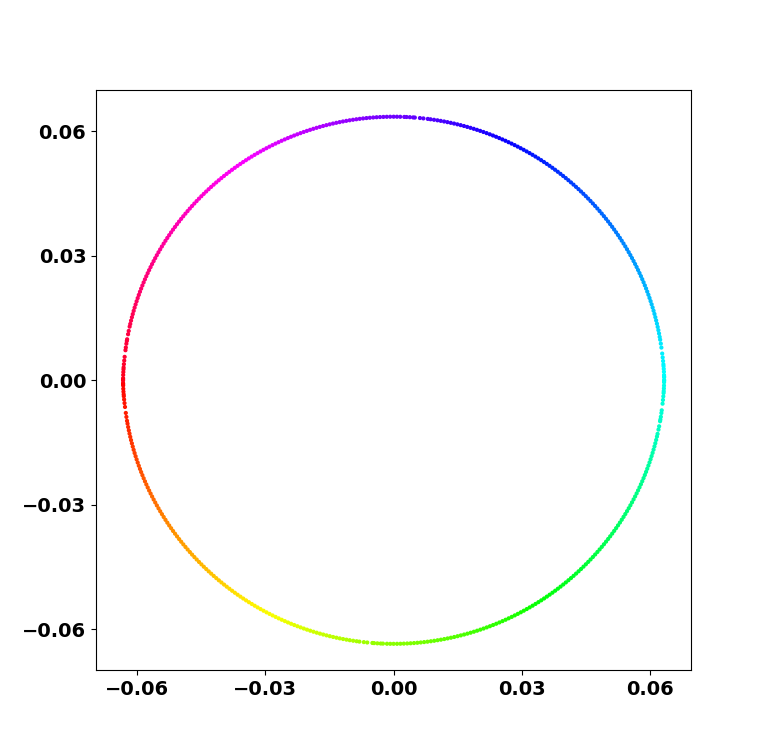
\includegraphics[width=\textwidth]{phaton_clean_manifold_500_k6.png}
      \caption{Clean sinogram GL-manifold, $k = 6$ and 500 samples.}
      \label{fig:clean_manifold_500}
    \end{subfigure}\hfill
    \caption{Shepp-Logan phantom sinogram GL embeddings: Importance of number of samples}
  \end{figure}


Moreover, the number of sampling points is important as well.
For more sampling points it is expected to be harder to come up with good neighbors (fixing k and number of samples),
as more data need to be explained with the same amount of neighbors, and it is more likely, that nodes are connected wrongly.
This can be seen in Figure~\ref{fig:clean_manifold_res200} and Figure~\ref{fig:clean_manifold_res400}, where with $dim(s) = 200$,
the perfect circle can be established and with $dim(s) = 400$, not anymore (by same parameter $k = 6$ and $\theta \in \mathbb{R}^{500}$).

\begin{figure}[H]
    \centering
    \hfill
    \subbottom[\label{fig:clean_manifold_res200}]
        {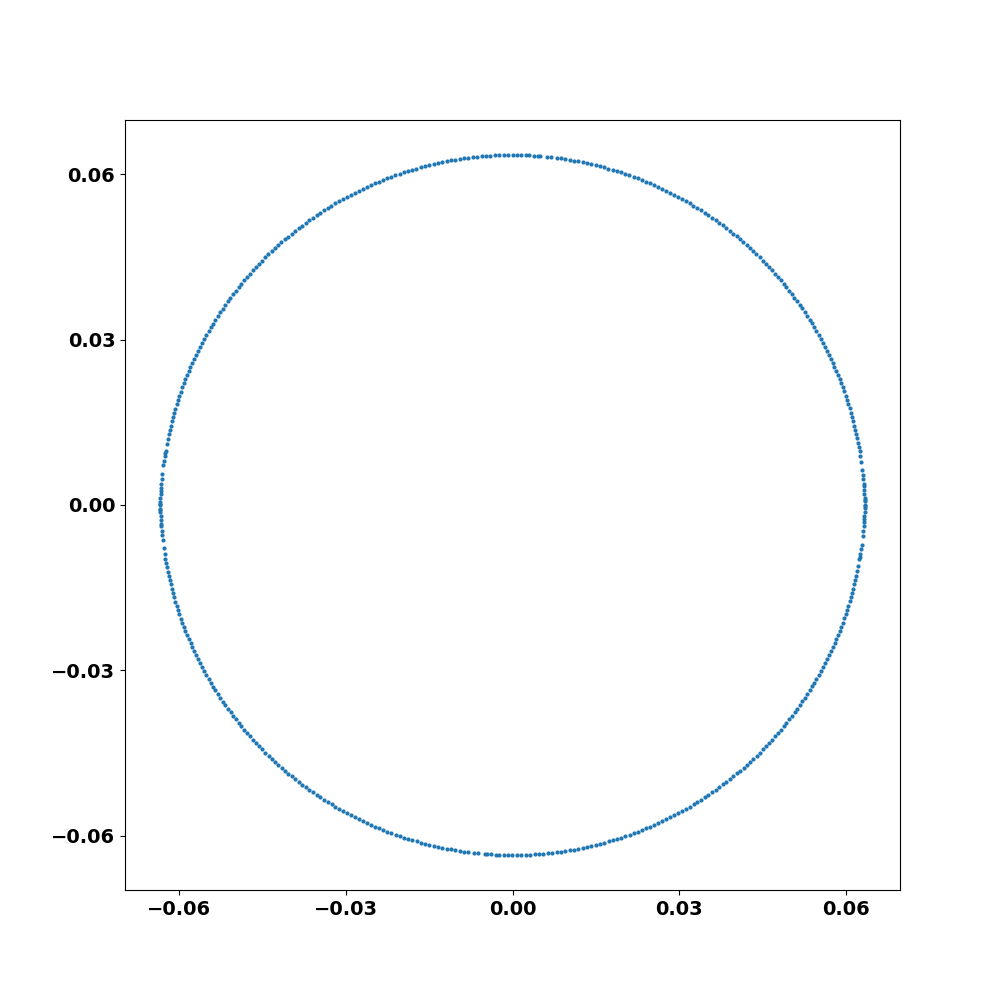
\includegraphics[width=0.4\textwidth]{phaton_clean_manifold_res_200_k6.png}}
    \hfill
    \subbottom[\label{fig:clean_manifold_res400}]
        {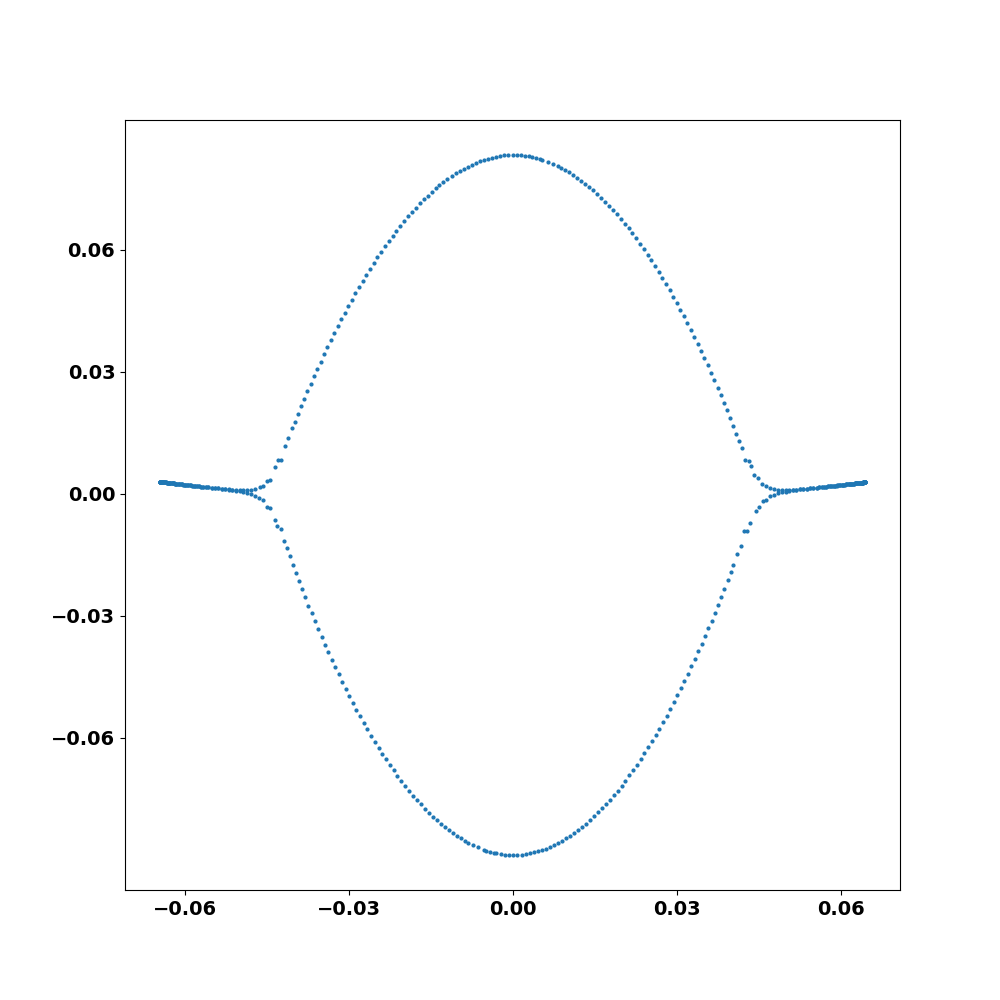
\includegraphics[width=0.4\textwidth]{phaton_clean_manifold_res_400_k6.png}}
    \hfill
    \caption{Shepp-Logan phantom sinogram GL-manifolds: Importance of number of samples.
    \ref{fig:clean_manifold_res200} Clean sinogram GL-manifold, $k = 6$ and $\text{resolution}=200$,
    \ref{fig:clean_manifold_res400} Clean sinogram GL-manifold, $k = 6$ and $\text{resolution}=400$}
\end{figure}


\begin{tcolorbox}[colback=red!5!white,colframe=red!75!black]
    Since the GL-manifold is sensitive to $k$, it is best practice to try different values in order to find the best GL-manifold.
\end{tcolorbox}





 
	\chapter{Neural Networks}
\label{sec:neural_networks}
In GAT-Denoiser, concepts from existing neural networks have been used.
In this chapter, GAT, Convolution and U-Net are introduced in detail.

\section{Graph Attention Networks}
The main component of GAT-Denoiser is a GAT.
GAT is an extension to GCN and adds attention (or weights) to neighbors for learning new node feature representations. 
Topology of the graph will not change but weighted averaging over the neighborhood will be computed.

\paragraph{Single Layer}
Input of a single GAT layer are node features $h = \{ h_1, h_2, \dots , h_N \} \in \mathbb{R}^F$, 
where $N$ is the number of nodes and $F$ the number of features per node. 
Single layer will map input to output, which can potentially have different dimensions: 
$h^{\prime} = \{ h_1^{\prime}, h_2^{\prime}, \dots, h_N^{\prime} \} \in \mathbb{R}^{F^{\prime}} $
As is other GNNs, input features are initially linearly transformed and parametrized by a learnable weight matrix 
$W \in \mathbb{R}^{F^{\prime} \times F}$. 
This allows to add enough expressiveness to the neural network and weights are learned during training.
Further, attention coefficients are computed, which indicates importance of node $j$ to node $i$:

\begin{equation}
  e_{ij} = a(Wh_i, Wh_j)
\end{equation}

With $a$ as the shared attentional mechanism $a : \mathbb{R}^{F^{\prime}} \times \mathbb{R}^{F^{\prime}} \mapsto \mathbb{R}$.
\citet{GAT} proposed to use a single-layer feedforward neural network, parametrized by a weight vector $a \in \mathbb{R}^{2F^{\prime}}$
and LeakyReLu as activation function.

To compare coefficients $e$ across different nodes, normalization is needed.
Therefore, softmax is used as normalization $\alpha_{ij} = softmax_j(e_{ij})$ 
such that all attention coefficient of one node sum up to 1 and therefore are nicely comparable across nodes.
Finally, new node embedding is calculated as:

\begin{equation}
  h_i^{\prime} = \sigma \left( \sum_{j \in \mathcal{N}_i} \alpha_{ij} W h_j \right)
\end{equation}

With $\sigma$ as some arbitrary activation function.

\begin{figure}[H]
  \centering
  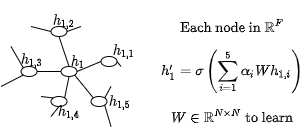
\includegraphics[width=0.6\textwidth]{GAT.drawio.png}
  \caption{GAT attention illustration example.}
  \label{fig:gat_attention_illustration}
\end{figure}


\paragraph{Multi-Head attention}
Motivated by the work of \citet{transformer}, multi-head attention can be beneficial to stabilize learning process.
Therefore, not only a single weight matrix is learned, but $W$ is split up in several parts, 
all learned individually:

\begin{equation}
  h_i^{\prime} = \bigparallel^K_{k=1} \sigma \left(\sum_{j \in \mathcal{N}_i} \alpha_{ij}^k W^k h_j \right),  
\end{equation}

Where $\parallel$ corresponds to concatenation, $\alpha_{ij}^k$ the $k$-th attention mechanism and $W^k$ the linear
transformations weight matrix. The final output consists of $KF^{\prime}$ output features.

\paragraph{Last layer:}
In the last layer, output dimension needs to be obtained. 
Consequently, concatenation is no longer plausible and averaging is used to match desired dimension.

\section{Convolution}
Convolution is an important part in Signal Processing, because it allows to average an incoming signal.
Convolution commonly operators on pixel spaces, where every observation location or time slot gets one value assigned.

\begin{equation}
  x \star k = y,
\end{equation}

Where $x$ is input signal, $k$ is kernel, $\star$ the convolution operator and $y$ the convolved signal.

To apply convolution, a kernel with weights needs to be defined. 
This kernel will then slide over the input signal $x$ and computes the dot product with its weights.
Figure~\ref{fig:1d-convolution} illustrates 1D convolution. Kernel size is set to 3, $n$ refers to input signal size and $m$ to output signal size.
In the example  $ n = m + 2$, thus, the convolved output signal size will be decreased by $2$.
The concept of convolution can be extended to arbitrary dimensions.

\begin{figure}[H]
  \centering
  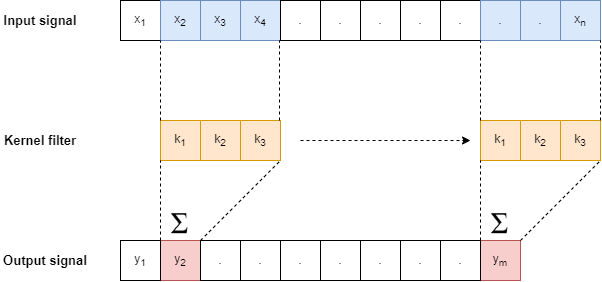
\includegraphics[width=0.6\textwidth]{Convolution.drawio.png}
  \caption{1D Convolution}
  \label{fig:1d-convolution}
\end{figure}

\paragraph{Padding:} 


Padding can be defined to add pixels to boundary of the signal.
In the example, padding is set to $0$ and therefore, the signal size is decreased by $2$.
If signal size should be fixed during convolution, padding is a powerful tool. For padding $1$,
the input size $n$ would be equal to output size $m$, as an extra element in the output signal
will be at convolved at boundaries.


\paragraph{Stride:}
Stride is the parameter how far kernel moves each time. In the example, stride was defined to be $1$.
If stride is increased, the output signal size will decrease.

\section{U-Net}
\label{sec:unet}
U-Net can boost performance of CT reconstruction, where FBP is further refined with a neural network.
It is a convolutional neural network, which is well suited for image segmentation in different domains.
\cite{unet-tomography} showed great success for biomedical image segmentation.

The neural network architecture consists of contracting path and expansive path,
resulting in a U-shape, as illustrated in Figure~\ref{fig:u-net-architectue}.

\begin{figure}[H]
  \centering
  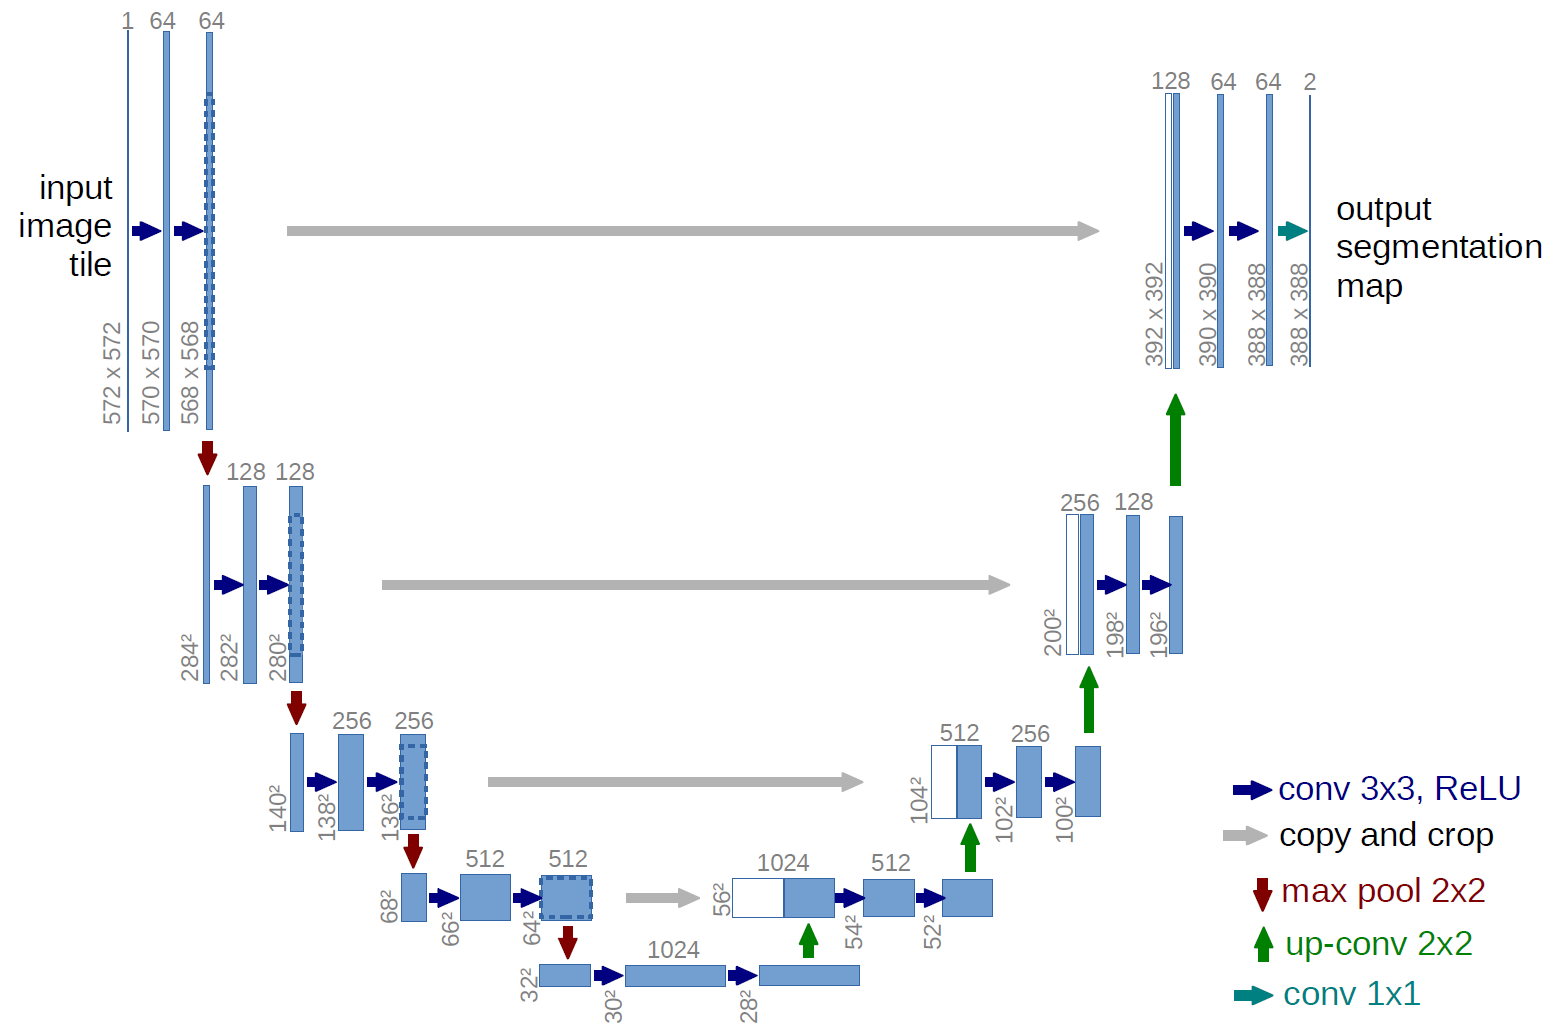
\includegraphics[width=0.6\textwidth]{u-net-architecture.png}
  \caption{
    U-Net architecture \cite[p 2, Fig. 1]{unet-tomography} \\
    Number on top of boxes denotes channels, where numbers at bottom of boxes refer to input dimension.
    }
    \label{fig:u-net-architectue}
\end{figure}


During contracting path (left part), input dimension is decreased but channels increased.
For every step in the contracting path, two 3x3 convolution layers are followed by ReLu
and a 2x2 max pooling for down-sampling. Further, at each down-sampling step, input channels are doubled.
Multiple contracting steps are combined. After last contracting step, expansive path (right part) starts
where input dimension will be increased and input channels will be decreased.
For every expansive step, an up-sampling of the feature map takes place, followed by a 2x2 convolution, 
which halves the number of channels. Then, concatenation with the corresponding feature
map of the contracting path is done (gray arrow in Figure~\ref{fig:u-net-architectue}), followed by again two 3x3 convolutions and ReLu.
Final layer is a 1x1 convolution to map to desired output dimension and single output channel.

 
	% !TEX root = ../Thesis.tex

\chapter{Additional Results}
In this chapter, additional numeric and visual results are presented, that shall
extend results presented in Chapter~\ref{sec:results}.

\section{Small Scale Experiment: GAT-Denoiser Components}

Table~\ref{tab:small_gat_components} shows numerical results for the small scale experiment.
Results for the baseline algorithms, different models with $k=2$ and $k=8$ are presented.  
\begin{table}[H]
    \centering
    \begin{tabular}{l|c|c|c|c}
      \toprule
      \textbf{Algorithm / Model} & \snrh{0} & \snrh{-5} & \snrh{-10} & \snrh{-15} \\
                         & \small \textbf{SNR} & \small \textbf{SNR} & \small \textbf{SNR}  & \small \textbf{SNR} \\ 
      \midrule
      FBP                 & 4.50 & -0.31  & -5.25 & -10.22  \\ \hline
      BM3D sino           & 9.93 &  7.42  & 4.61  & \textbf{2.00 }   \\ \hline
      BM3D reco           & \textbf{10.79} & \textbf{8.09}  &\textbf{ 4.97}  & 1.54    \\ \hline
      U-Net               & 7.13  &  6.18 & 4.34  & 1.87    \\ \hline
      \midrule
      \multicolumn{5}{c}{\textbf{k=2}} \\
      GAT             &	9.42 	&8.25	&6.78	&5.75  \\  \hline
      Conv+GAT        & 10.01 &8.88	&7.69	&6.79  \\ \hline
      GAT+U-Net       &	7.93	&7.28	&6.77	&4.91  \\ \hline
      GAT+U-Net*      &	11.92	&10.14	&10.13	&8.43 \\ \hline
      GAT+U-Net**     &	\textbf{13.41	}&\textbf{12.12}	&10.62	&8.50  \\ \hline
      Conv+GAT+U-Net  &	8.17	&7.09	&4.53	&5.67  \\ \hline
      Conv+GAT+U-Net* &	12.60	&10.71	&8.80	&8.44  \\ \hline
      Conv+GAT+U-Net**&	12.80	& 11.70	&\textbf{10.63}	&\textbf{9.21} \\ \hline
      
      \midrule
      \multicolumn{5}{c}{\textbf{k=8}} \\
      GAT                  & 8.32           & 6.94           & 6.19 & 5.01 \\ \hline
      Conv+GAT           & 9.05           & 8.07           & 6.99  & 5.75 \\ \hline
      GAT+U-Net          & 7.49           & 6.40           & 6.01   & 5.07 \\ \hline
      GAT+U-Net**        & 11.88          & \textbf{10.85} & \textbf{9.68} & \textbf{8.26} \\ \hline
      Conv+GAT+U-Net   & 7.55           & 6.50           &5.74 &4.87 \\ \hline
      Conv+GAT+U-Net** & \textbf{11.94} & 10.31          &7.34   &7.33 \\ \hline
      \midrule
    
    \end{tabular}
    % \legend{The evaluated GAT-Denoiser models have been trained with 1024 images for 200 epochs. 
    % U-Net* refers to joint U-Net training and U-Net** to joint U-Net training, after a 
    % training of 100 epochs of GAT-Denoiser alone. }
    \caption{Small Scale Experiment: GAT-Denoiser components vs. baseline algorithms.}
    \label{tab:small_gat_components}
  \end{table}


\section{Small Scale Experiment: Further k-NN Results}
K-NN experiment with 2 layers and 4 heads can be found in Table~\ref{tab:small_knn_2}. 

\begin{table}[H]
  \centering
  \begin{tabular}{l|cc}
    \toprule
    \small\textbf{k} & \multicolumn{2}{c}{\snrh{0}}   \\
                       & \small \textbf{Loss} & \small \textbf{SNR}  \\ 
    \midrule
    2    & \textbf{9.90} & \textbf{601.4}  \\ \hline
    4    & 9.64 & 622.1  \\ \hline
    6    & 9.38 & 634.4  \\ \hline
    8    & 9.19 & 649.0  \\ \hline
    \midrule
  \end{tabular}

  \caption{Small Scale Experiment: Different $k$ values for \snry 0 dB.}
  \label{tab:small_knn_2}
\end{table}


\section{Small Scale Experiment: GAT Dropout}
Table~\ref{tab:small_dropout} presents results for experiments with different dropout values.
GAT-Denoiser was defined with 2 layers and 4 heads.

\begin{table}[H]
  \centering
  \begin{tabular}{l|cc}
    \toprule
    \small \textbf{GAT dropout} & \multicolumn{2}{c}{\snrh{-5}}   \\
                       & \small \textbf{Loss} & \small \textbf{SNR}  \\ 
    \midrule
    0       & \textbf{8.33} & \textbf{739.5}  \\ \hline
    0.01    & 7.81 & 766.2  \\ \hline
    0.03    & 7.98 & 743.3  \\ \hline
    0.05    & \textbf{8.09} & \textbf{738.4}  \\ \hline
    0.1     & 7.79 & 761.8  \\  \hline
    \midrule
  \end{tabular}

  \caption{Small Scale Experiment: GAT dropout for \snry -5 dB.}
  \label{tab:small_dropout}
\end{table}

\clearpage
\section{Large Scale Experiment: Baseline Results}
Table~\ref{tab:baseline-large} presents the result of the chosen baseline algorithms
for the large scale experiment.

\begin{table}[H]
  \centering
  \begin{tabular}{l|cc|cc|cc|cc}
    \toprule
    \small\textbf{Algorithm} & \multicolumn{2}{c|}{\snrh{0}} & \multicolumn{2}{c|}{\snrh{-5}} & \multicolumn{2}{c|}{\snrh{-10}} & \multicolumn{2}{c}{\snrh{-15}} \\
                       & \small \textbf{Loss} & \small \textbf{SNR} & \small \textbf{Loss} & \small \textbf{SNR} & \small \textbf{Loss} & \small \textbf{SNR} & \small \textbf{Loss} & \small \textbf{SNR} \\ 
    \midrule
    FBP                 & 4.57  & 1167.6 & -0.19 & 1973.5 & -5.17 & 3425.3 & -10.09 & 10'737.3       \\ \hline
    BM3D sino           & 9.93  & 709.9  &  7.40 & 890.6  & 4.61  & 1168.0 & \textbf{2.09}   & \textbf{1570.0} \\ \hline
    BM3D reco           & \textbf{10.85} & \textbf{658.2}  & \textbf{8.15}  &\textbf{ 818.6}  & \textbf{5.07}  & \textbf{1118.3} & 1.76   & 1662.5 \\ \hline
    U-Net               & 7.18  &  968.8 & 6.34  & 1044.7 & 4.50  & 1214.1 & 1.94   & 1522.4        \\  \hline
    \midrule
  \end{tabular}
  \caption{Large Scale Experiment: Baseline results.}
  \label{tab:baseline-large}
\end{table}

\subsection{Large Scale Experiment: GAT-Denoiser Models}
Table~\ref{tab:large_gat_components_knn2} presents the final results for baseline algorithms
and GAT-Denoiser models for the large scale. 

\begin{table}[H]
    \centering
    \begin{tabular}{l|c|c|c|c}
      \toprule
      \small\textbf{Algorithm / Model} & \snrh{0} & \snrh{-5} & \snrh{-10} & \snrh{-15} \\
                         & \small \textbf{SNR} & \small \textbf{SNR} & \small \textbf{SNR}  & \small \textbf{SNR} \\ 
      \midrule
      FBP                 & 4.57   & -0.19  & -5.17  & -10.09 \\ \hline
      BM3D sino           & 9.93   &  7.40  & 4.61   & \textbf{2.09}   \\ \hline
      BM3D reco           & \textbf{10.85}  & \textbf{8.15}   & \textbf{5.07}   & 1.76   \\ \hline
      U-Net               & 7.18   & 6.34   & 4.50   & 1.94   \\  \hline
      \midrule
      \multicolumn{5}{c}{\textbf{k=2}} \\
    
        GAT              & 9.36	& 7.89	& 6.64	& 5.32    \\ \hline
        Conv+GAT         &	10.05	& 9.07	& 7.17	& 6.15    \\ \hline
        GAT+U-Net        &	8.39 	& 7.49	& 6.60	& 5.66    \\ \hline
        GAT+U-Net**      &	13.34	& 12.07	& \textbf{11.46}	& \textbf{9.62}   \\ \hline
        Conv+GAT+U-Net   &	8.31	& 7.47	&6.66	  & 5.15   \\ \hline
        Conv+GAT+U-Net** &	\textbf{13.43}	& \textbf{12.52}	& 11.43	& 9.55   \\ \hline
        \midrule
    \end{tabular}
  
    \caption{Large Scale Experiment: GAT-Denoiser components vs. baseline algorithms.}
    \label{tab:large_gat_components_knn2}
  \end{table}

\clearpage
\section{Large Scale Experiments: Visual Results}
\label{sec:large_scale_visual_results}
In this section, further visual results for the large scale experiment are presented for 
\snry 0 dB, -5 dB, -10 dB and -15 dB.
Clean images are repeated at every subsection, even tough they are the same.

\subsection{\snry 0 dB}
\visualresults{0}

\clearpage

\subsection{\snry -5 dB}
\visualresults{-5}

\clearpage

\subsection{\snry -10 dB}
\visualresults{-10}

\clearpage
\subsection{\snry -15 dB}
\visualresults{-15}

\clearpage
\section{Wandb Results}
\label{sec:wandb}
Table~\ref{tab:wandb_results} shows urls raw wandb results for all computed experiments on the LoDoPaB-CT dataset.
\begin{table}[H]
  \centering
  \begin{tabular}{l|l}
    \toprule
    \textbf{Experiments} & \textbf{URL} \\ 
    \midrule
    \multicolumn{2}{c}{\textbf{Small Scale Experiments:}} \\
    FBP & \url{https://wandb.ai/cedric-mendelin/FBP-Validation-LoDoPaB-small} \\ \hline
    BM3D & \url{https://wandb.ai/cedric-mendelin/BM3D-Validation-LoDoPaB-small} \\ \hline
    U-Net& \url{https://wandb.ai/cedric-mendelin/U-Net-Validation-LoDoPaB-small} \\ \hline
    K-nn &\url{https://wandb.ai/cedric-mendelin/LoDoPaB-Small-k-NN-and-graph-size} \\ \hline
    Convolution & \url{https://wandb.ai/cedric-mendelin/LoDoPaB-Small-Convolution} \\ \hline
    Loss& \url{https://wandb.ai/cedric-mendelin/LoDoPaB-Small-Loss-FBP-vs-SINO} \\ \hline
    GAT dropout& \url{https://wandb.ai/cedric-mendelin/LoDoPaB-Small-GAT-dropout} \\ \hline
    GAT-Denoiser $k=2$ & \url{https://wandb.ai/cedric-mendelin/LoDoPaB-Small-Components-knn-2} \\ \hline
    GAT-Denoiser $k=8$ & \url{https://wandb.ai/cedric-mendelin/LoDoPaB-Small-Components-knn-8} \\ \hline
    \midrule
    \multicolumn{2}{c}{\textbf{Large Scale Experiments:}} \\
    U-NET & \url{https://wandb.ai/cedric-mendelin/U-Net-Validation-LoDoPaB-large} \\ \hline
    FBP& \url{https://wandb.ai/cedric-mendelin/FBP-Validation-LoDoPaB-large} \\ \hline
    BM3D& \url{https://wandb.ai/cedric-mendelin/BM3D-Validation-LoDoPaB-large} \\ \hline
    GAT-Denoiser & \url{https://wandb.ai/cedric-mendelin/LoDoPaB-Large-knn-2} \\ \hline
    \midrule

  \end{tabular}
  \caption{Wandb raw results.}
  \label{tab:wandb_results}
\end{table}

\paragraph{Average Wandb Run Result:}
Average SNR and loss have been computed with a python script and exported values can be found under\footnote{https://github.com/cedricmendelin/master-thesis/tree/main/wandb\_results}.
 
\end{appendices}
\addtocontents{toc}{\protect\setcounter{tocdepth}{2}}
%% ----------------------------------------------------------------
\thesisback
%\iflanguage{english}
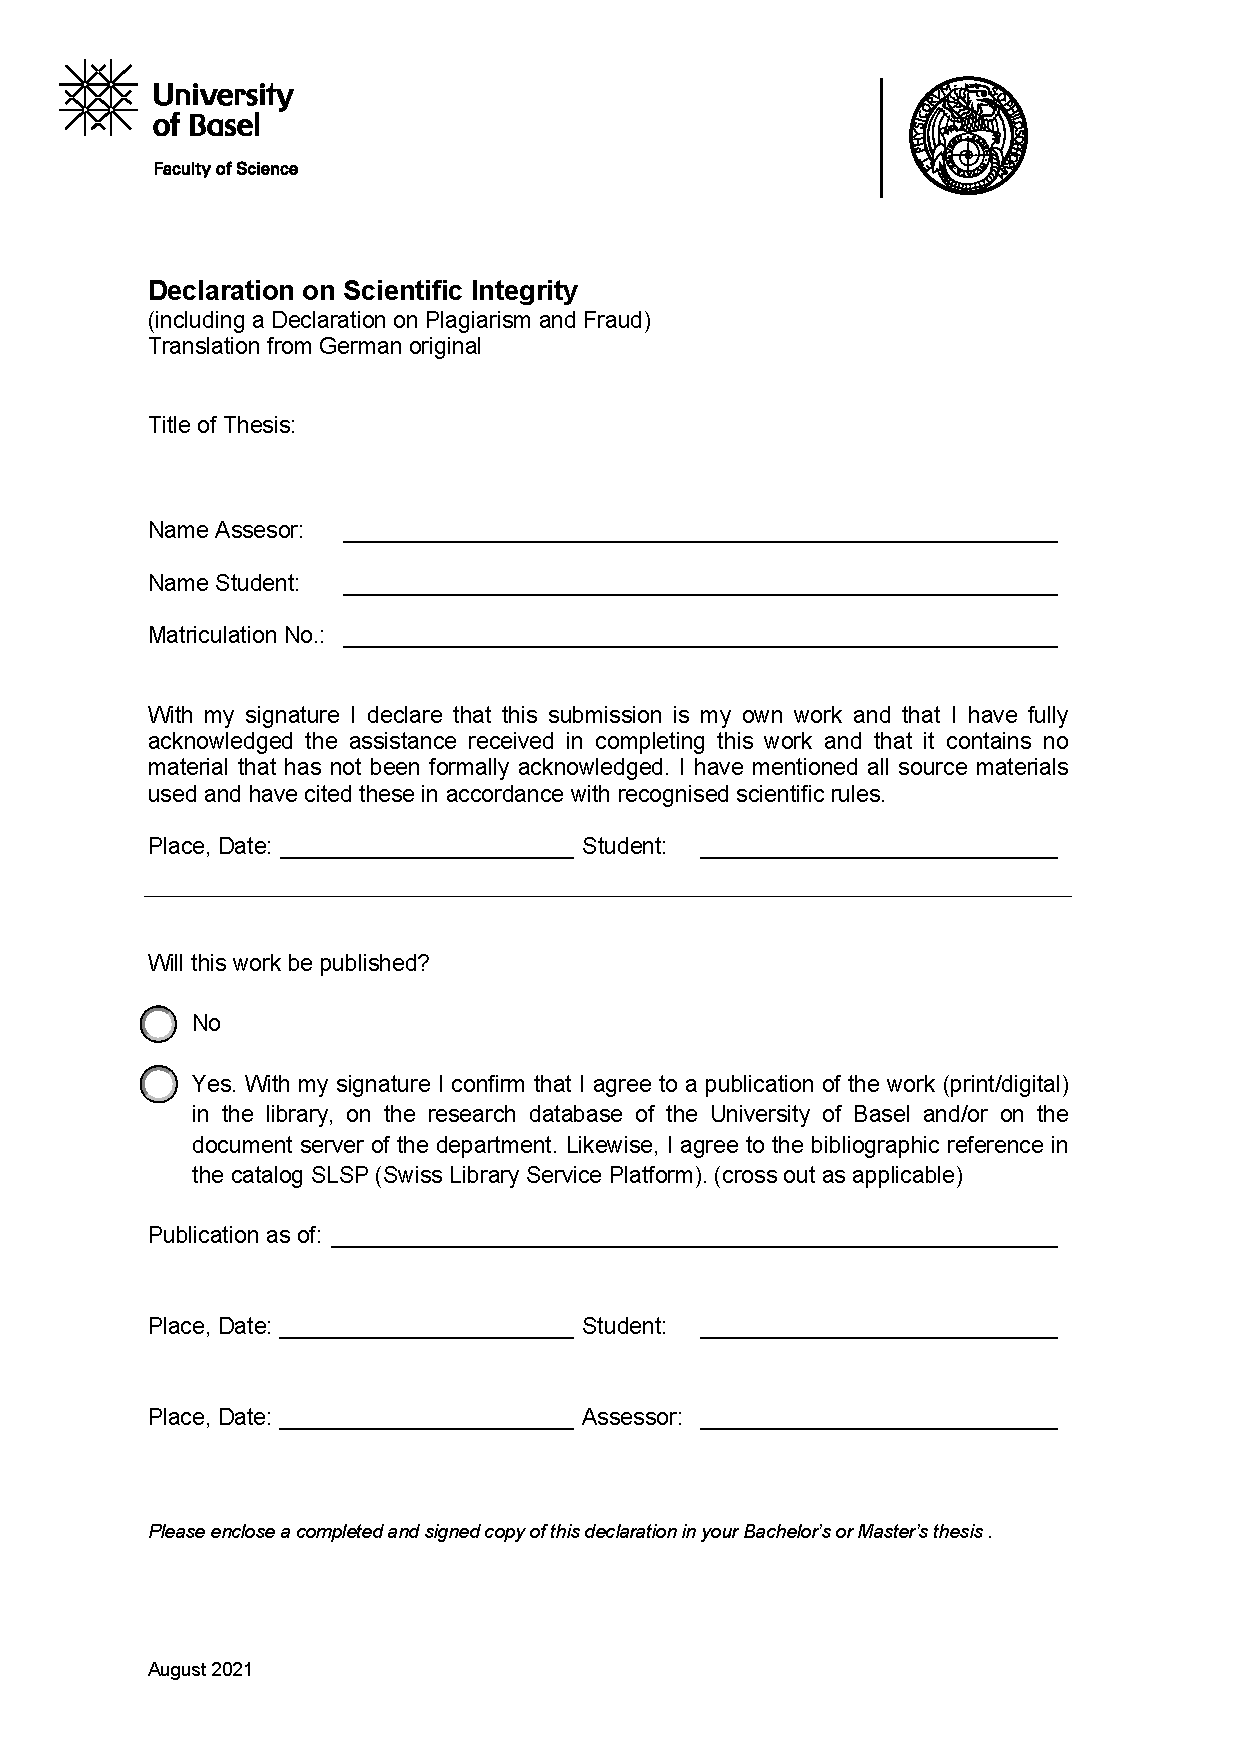
\includepdf{./Back/wissensch_Redlichkeit_E_Aug_21.pdf}
{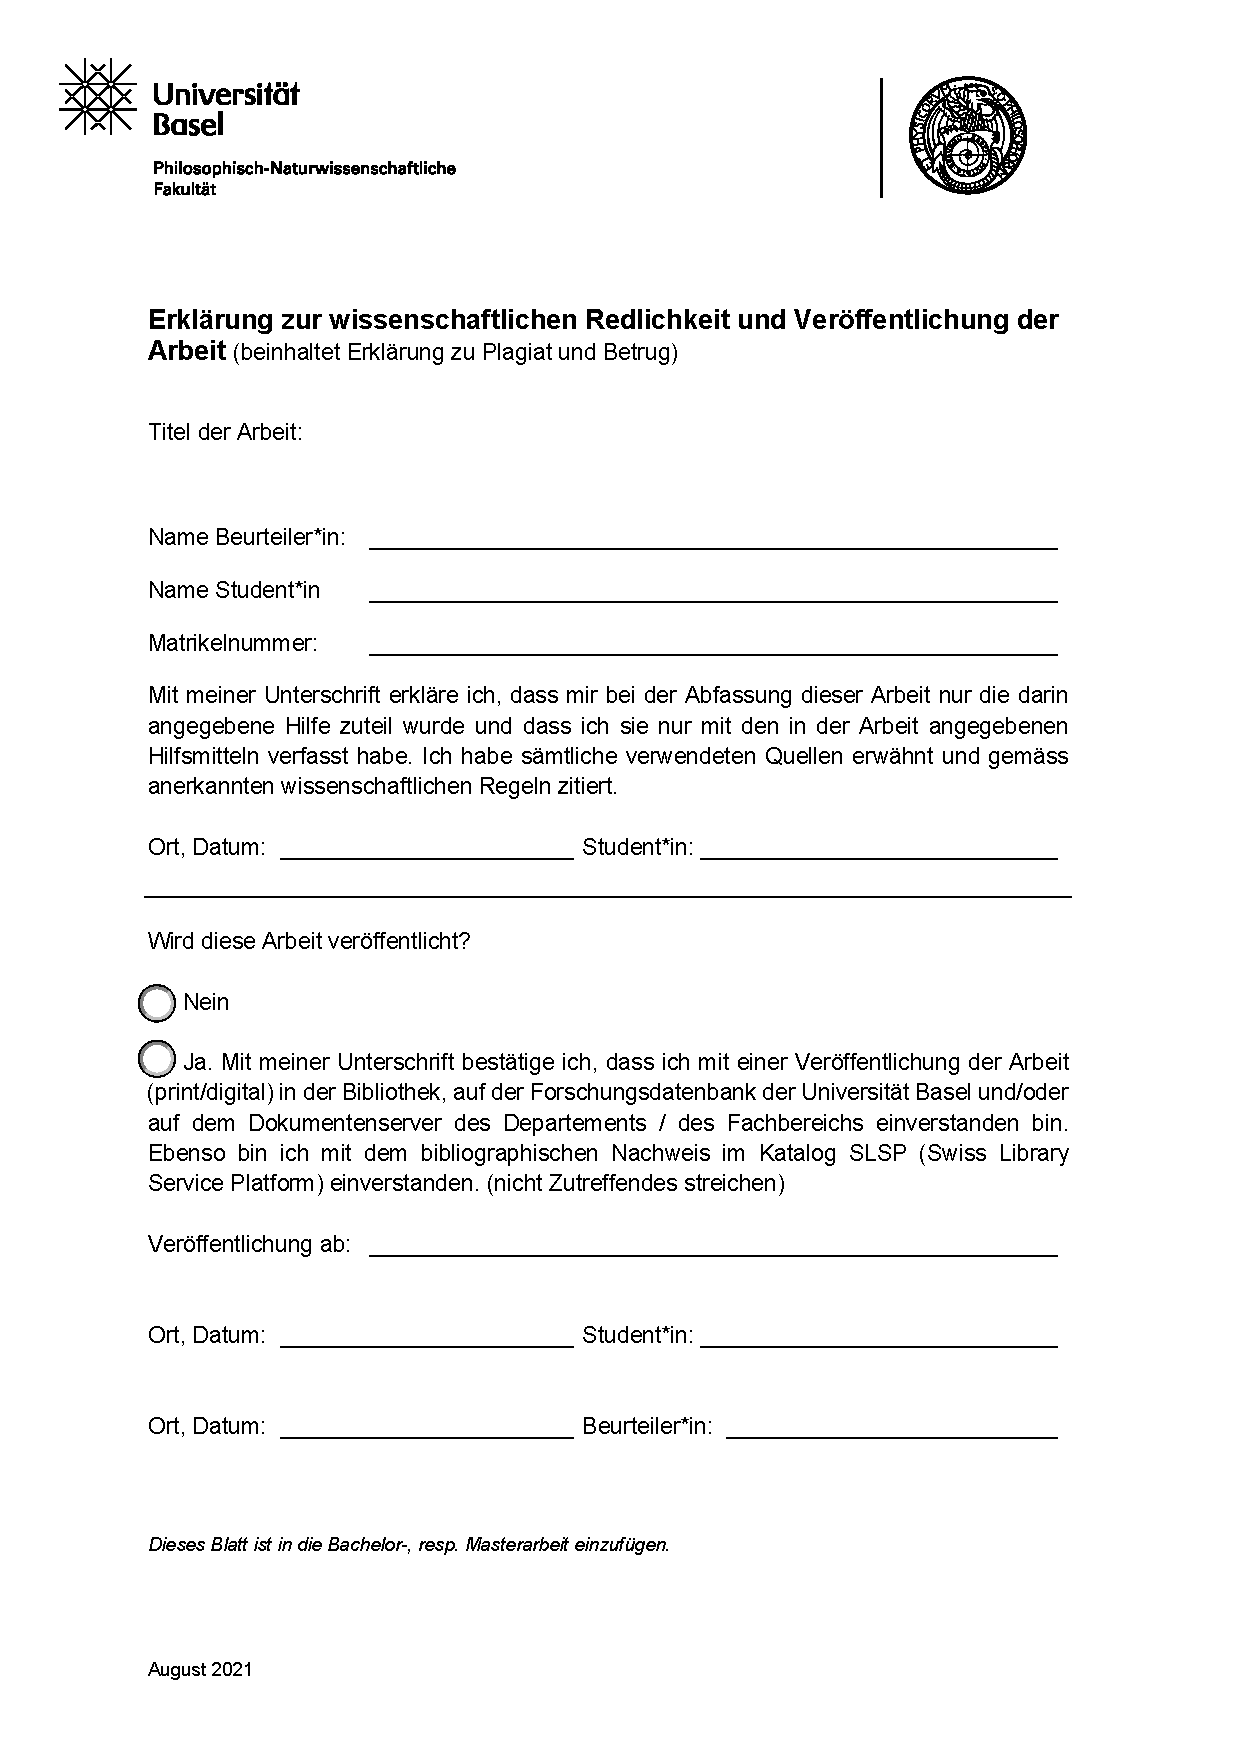
\includepdf{./Back/wissensch_Redlichkeit_D_Aug_21.pdf}}
%% ----------------------------------------------------------------
\end{document}
%% ----------------------------------------------------------------
